\section{Contextualização do Problema e Justificativa}

O presente estudo tem como objetivo analisar a existência de vieses de julgamento na população geral e como esses vieses influenciam as escolhas políticas e econômicas. A pesquisa parte da premissa de que as crenças econômicas dos eleitores são frequentemente enviesadas, resultando em decisões políticas potencialmente sub-ótimas para o desenvolvimento econômico e social.

Além disso, é fundamental examinar a interação entre o Estado e a sociedade civil, considerando como essa dinâmica pode influenciar os vieses de julgamento. A relação entre a autoridade estatal e a capacidade de auto-organização da sociedade pode criar um ambiente que exacerba ou mitiga esses vieses. Nesse sentido, o equilíbrio entre a autoridade estatal e a liberdade individual é crucial para a formação das crenças e decisões políticas e econômicas dos cidadãos \cite{acemoglu2019narrow}.

Ademais, as teorias econômicas e a disseminação de conhecimento econômico desempenham um papel significativo na formação das crenças dos eleitores. A complexidade do pensamento econômico e as dificuldades na transmissão acessível dessas ideias ao público geral podem resultar em interpretações enviesadas que afetam diretamente as escolhas eleitorais e políticas. Neste contexto, as ideias de Bryan Caplan sobre o irracionalismo dos eleitores destacam como as preferências sistematicamente enviesadas podem distorcer o processo democrático e as políticas públicas \cite{The_Myth_of_the_Rational_Voter}.

Assim, este estudo não apenas investiga a presença de vieses de julgamento, mas também explora a interseção entre fatores históricos, sociais e econômicos que contribuem para a formação dessas crenças. Ao compreender essas interações complexas, podemos obter insights valiosos sobre como melhorar a educação econômica e promover decisões políticas mais informadas e eficazes, visando o progresso econômico e social.

Além disso, este trabalho contribui para o enriquecimento de uma nova área de estudo denominada "economia política comportamental". Essa área de pesquisa emergente busca integrar princípios da economia, ciência política e psicologia comportamental para entender melhor como os indivíduos tomam decisões econômicas e políticas e como esses processos podem ser influenciados por diversos fatores contextuais e cognitivos.

O método usado para a análise do presente trabalho será de revisão bibliográfica de várias fontes e análises empíricas já realizadas. A análise dos vieses de julgamento será feita a partir de uma abordagem interdisciplinar, considerando insights da economia comportamental, ciência política e história econômica. A pesquisa buscará identificar padrões e tendências nos vieses de julgamento e suas implicações para a democracia e as políticas públicas.

\section{Fundamentos Teóricos }

A análise dos fundamentos teóricos e das evidências empíricas na economia política comportamental é crucial para entender como os indivíduos tomam decisões econômicas e políticas. A economia comportamental, ao integrar conceitos da psicologia, desafia a noção tradicional de que os agentes econômicos são perfeitamente racionais e maximizadores de utilidade. Este campo de estudo examina como fatores cognitivos, emocionais e sociais influenciam as escolhas individuais e coletivas, oferecendo uma visão mais realista do comportamento humano.

Pesquisas têm demonstrado que as decisões dos eleitores e formuladores de políticas são frequentemente influenciadas por vieses cognitivos e heurísticas, que podem levar a escolhas sub-ótimas tanto no contexto econômico quanto no político. Esses vieses são moldados por diversos fatores, incluindo experiências passadas, influências culturais e a estrutura institucional na qual os indivíduos estão inseridos \cite{The_Myth_of_the_Rational_Voter, Systematically_Biased_Beliefs_about_Economics, saee1996}. 

A economia política comportamental emergiu como uma área de estudo promissora que busca entender essas dinâmicas complexas. Ao combinar insights da economia comportamental e da ciência política, essa disciplina oferece ferramentas valiosas para analisar como as crenças e atitudes dos eleitores impactam o funcionamento das democracias e a implementação de políticas públicas.


\subsection{O pensamento de economista} 
% o que caracteriza o pensamento de economista segundo a literatura, abordando a racionalidade, a busca por eficiência e a importância da informação.
% como o pensamento do economista se difere das percepções comuns da população comum.

Os economistas no geral operam sob o pressuposto de que os agentes econômicos são racionais e buscam maximizar sua utilidade ou satisfação a partir das escolhas disponíveis, o famoso "Homo Economicus". Esta abordagem implica que os indivíduos tomam decisões de forma lógica e consistente, com base nas informações disponíveis e a partir de uma avaliação cuidadosa das alternativas. É crucial também destacar a importância do pensamento da racionalidade das decisões econômicas, onde se argumenta que o comportamento racional é essencial para a eficiência e a eficácia das políticas econômicas \cite{Hausman_McPherson_Satz_2016}.

A análise de custo-benefício é uma ferramenta central no pensamento dos economistas. Ela permite a avaliação das opções de decisão com base nos custos e benefícios associados, assegurando que as decisões sejam eficientes e justas \cite{KenBinmore2008}. Os economistas utilizam essa abordagem para formular políticas que maximizem o bem-estar social, equilibrando os custos e benefícios de cada intervenção.


A informação desempenha um papel crucial nas decisões econômicas. Economistas acreditam que decisões de alta qualidade dependem da disponibilidade e do uso eficaz da informação, argumentando que a coleta, a análise e a disseminação de dados são fundamentais para o funcionamento eficiente dos mercados e das políticas públicas \cite{positive_economics_friedman}. Desde os anos 30, Friedrich Hayek tem destacado a importância da alocação do conhecimento na sociedade. Em seu artigo seminal de 1945, Hayek argumentou que o principal problema econômico enfrentado pela sociedade não é a alocação de recursos dados entre fins concorrentes, mas sim como assegurar o melhor uso dos recursos conhecidos por qualquer membro da sociedade, para fins cuja importância relativa apenas esses indivíduos conhecem \cite{hayek_knowledge_use}. Ele também enfatizou que a dispersão e a imperfeição de todo o conhecimento são fatos básicos com os quais as ciências sociais devem começar \cite{hayek_knowledge_dispersion}. No entanto, as limitações cognitivas dos indivíduos e a quantidade limitada de informação disponível podem levar a decisões sub-ótimas, conforme destacado por Daniel Kahneman em sua obra sobre heurísticas e vieses \cite{Judgment_under_Uncertainty}.

O pensamento econômico difere significativamente das percepções comuns da população. Enquanto os economistas enfatizam a racionalidade, a análise de custo-benefício e a importância da informação, a população frequentemente baseia suas decisões em heurísticas e vieses. Essas heurísticas são regras simples e intuitivas que as pessoas usam para tomar decisões rápidas e, embora úteis em muitos contextos, podem levar a erros sistemáticos \cite{Judgment_under_Uncertainty}. A população também é influenciada por crenças infundadas e emoções, o que pode resultar em decisões que não são necessariamente racionais ou eficientes do ponto de vista econômico \cite{thaler2016misbehaving}.

Em resumo, a abordagem de Gary Becker define o que hoje temos por regra atualmente:

\begin{citacao}
    \textit{Acho difícil acreditar que a maioria dos eleitores seja sistematicamente enganada quanto aos efeitos de políticas como a de quotas e tarifas de importações que persistem há tempos. Prefiro supor que o eleitor tem expectativas não enviesadas, ao menos, quanto a essas políticas persistentes. Eles talvez superestimem o peso-morto de algumas medidas e subestimem o de outras, mas, em média, eles tem uma ideia correta.
    } \newline \cite{becker1976}
\end{citacao}

\subsection{Economistas e os Vieses de Julgamento nos Eleitores}
% Fazer uma introdução igual Caplan faz no livro dele, falando sobre a importância da democracia e como ela depende de eleitores bem informados e racionais.

A democracia se fundamenta na ideia de que eleitores informados e racionais são capazes de tomar decisões que promovem o bem-estar coletivo e o desenvolvimento sustentável. Em "The Myth of the Rational Voter", Caplan argumenta que a eficácia da democracia depende criticamente da capacidade dos eleitores de avaliar políticas e candidatos de maneira objetiva e informada. Contudo, na prática, muitos eleitores sofrem de vieses de julgamento que distorcem suas percepções e decisões, resultando em escolhas que podem ser prejudiciais para a sociedade como um todo \cite{The_Myth_of_the_Rational_Voter}.

Acemoglu e Robinson, em "The Narrow Corridor", enfatizam que o engajamento político ativo e informado da população é crucial para manter o equilíbrio entre a autoridade estatal e a liberdade individual. Eles argumentam que a capacidade da sociedade de se organizar e participar ativamente nos processos políticos é fundamental para evitar a tirania e promover políticas que refletem verdadeiramente as necessidades e interesses da população \cite{acemoglu2019narrow}.

No entanto, os vieses de julgamento nos eleitores podem comprometer esse ideal democrático. Esses vieses são frequentemente resultado de heurísticas cognitivas, que são atalhos mentais usados para simplificar a tomada de decisão, mas que podem levar a erros sistemáticos. Entre os principais vieses que afetam os eleitores estão:

\begin{enumerate}
    \item Viés antimercado
    \item Viés antiestrangeiro
    \item Viés antitrabalho
    \item Viés pessimista
\end{enumerate}

Essa lista provém de uma análise de Caplan, que argumenta que esses vieses são comuns entre os eleitores e podem resultar em políticas públicas ineficazes e prejudiciais. Ele destaca que a educação econômica e a disseminação de conhecimento são essenciais para combater esses vieses e promover decisões políticas mais informadas e eficazes \cite{The_Myth_of_the_Rational_Voter}.

Atualmente, o estudo da "Economia Política Comportamental" e seus vieses está sendo revitalizado. No entanto, é crucial lembrar que a história do pensamento econômico sempre foi marcada por discussões sobre esses temas e seus correlatos.

Muitos dos famosos economistas do passado, como Adam Smith e Fréderic Bastiat, eram obcecados pela moralidade e pelas crenças teimosas do povo quanto a economia, a sua insistente resistência  aos princípios básicos do custo de oportunidade e a vantagem comparativa \cite{hart2019bastiat,Wells2013,The_Myth_of_the_Rational_Voter}.

Parece que as os economistas tem se esquecido de que a economia é uma ciência social e que as pessoas são seres humanos, com crenças e valores que muitas vezes não se alinham com a lógica econômica. Questões que hoje são levantadas como novas, já foram a tempos levantadas por economistas como Bastiat, que em sua obra "O que se vê e o que não se vê" já discutia sobre a dificuldade de se perceber os custos ocultos das políticas públicas e como elas se comportam na subjetividade \cite{hart2019bastiat}.

Estudar mais a fundo esses vieses presentes nos eleitores, tendo como um grande aliado a história do pensamento econômico se faz mais necessário que nunca. Lembrando que o problema do tema não é que os economistas não tem nada a dizer sobre o assunto, mas sim que eles tem muito a dizer porém relutam a ir em público e arriscar a sua credibilidade científica. Se fosse possível superar essa relutância teríamos muito a dizer \cite{The_Myth_of_the_Rational_Voter}. Gustavo Franco pode elucidar essa parte como ninguém:

\begin{citacao}
    \textit{[...] Tenha claro, por favor, que não há problema nenhum em atacar a sabedoria estabelecida [...]. Mas não perca de vista que ir contra o senso comum é um esporte radical: há muito risco e, se você errar, vai acabar no hospital. Sempre é preciso provar o que você diz, e costuma ser difícil. [...] Muito cuidado ao atacar a sabedoria estabelecida, pois na maioria das vezes você estará errado. Lembre-se de que o conhecimento que você herda se estabeleceu do trabalho diligente de muitos como você e eu, depois de anos e anos de tentativa, erro e decantação. \newline
    }  \cite{franco2022cartas}
\end{citacao}

Então temos em nossas mãos um cenário muito otimista apenas de revelar o que os economistas já sabem. Poucos economistas contemporâneos se preocupam com a história do pensamento econômico, e isso é um erro, deixando muitas discussões importantes ignoradas ou esquecidas \cite{mark_history}. A história do pensamento econômico é uma disciplina que nos ajuda a entender como as ideias econômicas evoluíram ao longo do tempo e como elas moldaram a sociedade em que vivemos. Ela nos permite ver como as ideias econômicas foram influenciadas por eventos históricos, mudanças políticas e avanços tecnológicos, e como essas ideias continuam a influenciar o pensamento econômico contemporâneo.

Porém o foco aqui são os vieses que não podem ser ignorados, explicando eles com base em no que os economistas acreditam ser o certo ao longo da história documentada e em contraste o que a população no geral acredita. Provas formais dos vieses estarão mais a frente.


\subsubsection{Viés antimercado}
% Descreva como o viés antimercado leva os eleitores a desconfiarem das soluções de mercado, favorecendo intervenções estatais.

O viés antimercado pode ser resumido na tendência de subestimar os benefícios do mercado, de seus mecanismos de mercado e superestimar os custos associados a ele \cite{sowell2000basic,sowell2004applied,The_Myth_of_the_Rational_Voter}. 

O cidadão comum tende a acreditar que o mercado é ineficiente e injusto, tende a ter séria dúvidas de até onde pode confiar e contar com empresas lucrativas para gerar produtos socialmente benéficos. Se foca somente na motivação do lucro da empresa e é deixado de lado a parte da disciplina imposta pelo mercado, que faz com que empresas que não atendem as necessidades do consumidor sejam eliminadas do mercado. Os economistas no geral admitem que, a busca incessante pelo lucro aliada as falhas e imperfeições de mercado podem gerar resultados ruins, não-economistas veem a ganância bem sucedida como algo socialmente prejudicial por si só \cite{The_Myth_of_the_Rational_Voter}.

Shumpeter, em sua obra "Capitalismo, Socialismo e Democracia", define com perfeição esse viés:

\begin{citacao}
    \textit{O capitalismo é julgado por juízes que têm a sentença de morte preparada. Eles darão este veredito, não importa o que a defesa diga; a única coisa que a defesa pode fazer é provocar uma mudança na acusação. \newline
    }  \cite{schumpeter1976capitalism}
\end{citacao}

Essa visão de que o lucro é simplesmente uma forma de transferência, uma exploração e que o mercado é um jogo de soma zero, onde o ganho de um é a perda de outro, é um dos principais fatores que levam os eleitores a desconfiarem das soluções de mercado e a favorecerem intervenções estatais. Vale ressaltar que "transferência" no dialeto econômico é um termo que se refere a um movimento descompromissado de riqueza de um agente para outro, sem que haja um aumento na riqueza total da sociedade. Levando isso como base, podemos concluir que as pessoas tendem a ver os lucros como um presente para os mais ricos. Portanto, a não ser que o governo intervenha limitando os lucros como questão de bom senso, a riqueza não será redistribuída de forma justa e eficiente \cite{The_Myth_of_the_Rational_Voter}. Essa forma de pensar é exatamente o que Thomas Sowell chama de "raciocínio de estágio único", ou seja, considerar apenas as consequências imediatas e óbvias de uma medida, ignorando as consequências indiretas e menos óbvias \cite{sowell2004applied}.

É importante lembrar que o lucro não é uma esmola, mas sim um \textit{quid pro quo}: o lucro é a recompensa por atender as necessidades e desejos dos consumidores de forma eficiente e inovadora. O lucro é o sinal de que uma empresa está gerando valor para a sociedade, alocando os recursos de forma eficiente, e não um mecanismo de exploração. Essa é a lição básica que Adam Smith nos ensinou em "A Riqueza das Nações": a "mão invisível" do mercado, guiada pela busca do lucro, silenciosamente convence os empresários egoístas a servir o bem comum \cite{smith1776inquiry}.

Desde o início da história registrada também temos o lucro aparecendo de forma prejudicial, como o exemplo do lucro sobre o empréstimo de dinheiro, o juros, que era considerado pecaminoso e injusto. Desde a mesopotâmia até a igreja católica medieval, por exemplo, proibindo a cobrança de juros, considerando-a uma forma de exploração e usura \cite{tomasdeaquino_summa_78}. Eugen von Böhm-Bawerk consegue elucidar essa questão de forma clara em seu clássico "Capital e Juro":

\begin{citacao}
    \textit{O credor geralmente é rico e o devedor, pobre, e o primeiro parece um homem odioso que suga o pouco que o pobre tem na forma de juros e que pode aumentar ainda mais sua riqueza supérflua. Não é de se surpreender, contudo, que tanto a Antiguidade quanto a Idade Média Cristã viam com maus olhos os juros. 
    } \newline \cite{von2022capital}
\end{citacao}

Para encerrar esta parte mostrando a visão dos economistas, uma pessoa que ouça ou veja economistas discutindo questões como essa, como Krugman ou Stiglitz, pode ter a impressão de que a parte benéfica do mercado ainda é controversa ou não está acertada \cite{krugman2003great,stiglitz2003roaring,The_Myth_of_the_Rational_Voter}. Nesse ponto, é importante entender que os economistas não estão debatendo se os preços dão incentivos ou se há uma enorme conspiração para manter os preços altos. Eles estão simplesmente explicando como o mercado funciona. Quase todos os economistas reconhecem que o mercado é a melhor maneira de alocar recursos escassos e que a concorrência é a melhor maneira de garantir que os preços sejam justos e que os consumidores sejam protegidos; eles discordam apenas sobre o grau disso.

\subsubsection{Viés antiestrangeiro}
% Descreva como o viés antiestrangeiro leva os eleitores a desconfiarem de acordos comerciais e imigração, favorecendo políticas protecionistas e anti-imigração.

É sempre interessante começar a explicação de um tema começando com uma pergunta fundamental a ser respondida: Estrangeiros? Será que pe mesmo mutuamente benéfico comercializar com eles?

Uma frase de Alan Blinder pode começar a explicar o motivo dessa desconfiança:

\begin{citacao}
    \textit{
        Quando os empregos são escassos, o instinto de autopreservação ganha força e a tentação de culpar a concorrência estrangeira é irresistível. Não só nos Estados Unidos que a mentalidade protecionista ganhou peso. O fato de muitos economistas considerarem míope e um autoboicote o esforço de, por meio do protecionismo, salvar empregos não cabe aqui. Os legisladores estão aí para ganhar votos, não elogios de intelectuais.
     } \newline 
    \cite{blinder1987hard}
\end{citacao}

Para reforçar o discurso, nada melhor que o pai da economia moderna para também citar o que naquela época já era considerado reprovável:

\begin{citacao}
    \textit{
         De que vale a prudência na conduta de todas as famílias se a escassez pode ser enganada num grande reino? Se um país estrangeiro puder nos fornecer uma mercadoria por um preço mais baixo do que o nosso, melhor comprá-la com uma parte do produto da nossa indústria, empregando de forma a termos alguma vantagem.
    } \newline
    \cite{smith1776inquiry}
\end{citacao}

Os economistas criticam o viés antiestrangeiro porque ele não só está errada como também essa visão entra de conflito com a economia mais elementar ensinada nos primeiros meses de graduação. Os livros mais usados, como o de Mankiw, ensinam que o comércio é mutuamente benéfico, que a especialização e a troca aumentam a produtividade e o bem-estar de todos os envolvidos. Nas palavras dele, de seus dez princípios de economia, o número cinco é:

\begin{citacao}
    \textit{
        [...] É fácil se enganar, porém, ao pensar na competição entre países. O comércio entre os Estados Unidos e a China não é como uma competição esportiva, em que um lado ganha e o outro perde. De fato, o oposto é verdadeiro: o comércio entre dois países pode ser bom para ambas as partes.
    } \newline
    \cite{mankiw2020introducao}
\end{citacao}

A Lei das Vantagens Comparativas é o fenômeno que é descrito acima. Essa teoria, desenvolvida por David Ricardo, reforça ainda mais a importância do comércio internacional. Segundo Ricardo, mesmo que um país seja menos eficiente na produção de todos os bens em comparação a outro, ainda é vantajoso para ambos os países se especializarem na produção dos bens nos quais têm uma vantagem comparativa (ou seja, onde têm uma menor desvantagem relativa) e comercializarem entre si. Isso ocorre porque a especialização baseada nas vantagens comparativas maximiza a produção global e o bem-estar econômico \cite{ricardo1817principles}.

Além disso, políticas protecionistas frequentemente resultam em ineficiências econômicas e redução do bem-estar. O livre comércio permite que os países aproveitem suas vantagens comparativas, promovendo a eficiência e o crescimento econômico global \cite{bhagwati2003free}.

Outro exemplo de viés antiestrangeiro é a desconfiança em relação à imigração. Muitos eleitores acreditam que a imigração prejudica a economia local, aumenta a concorrência por empregos e recursos escassos e ameaça a identidade cultural. Os economistas de hoje reconhecem facilmente os benefícios da imigração. A troca de trabalho é praticamente a mesma que a troca de mercadorias. Especialização e a troca aumentam a produção e o bem-estar de todos os envolvidos. A imigração aumenta a força de trabalho, a produtividade e a inovação, impulsionando o crescimento econômico e a prosperidade.

Em síntese, o viés antiestrangeiro induz os eleitores a desconfiarem de acordos comerciais e imigração, resultando em políticas protecionistas e anti-imigração. No entanto, economistas sustentam que o comércio internacional e a imigração são vantajosos para a economia, promovendo eficiência, crescimento econômico e bem-estar global. Como ilustração final, Steven Landsburg elucida o comércio internacional comparando-o a uma tecnologia:

\begin{citacao}
    \textit{
        Há duas tecnologias para a produção de carros nos Estados Unidos. Uma delas é a manufatura em Detroit e a outra é a agricultura em Iowa. Todos conhecem a primeira; deixe-me falar da segunda. Primeira você planta as sementes, que são a matéria-prima dos carros. Você espera alguns meses até o trigo crescer. Daí você colhe o trigo, põe em navios e coloca os navios para cruzarem o Oceano Pacífico. Depois de alguns meses, os navios aparecem com Toyotas dentro deles.
    } \newline
    \cite{landsburg2012armchair}
\end{citacao}


\subsubsection{Viés antitrabalho}
% Discuta como o viés antitrabalho leva a uma resistência às mudanças tecnológicas e inovações. 

\begin{citacao}
    \textit{
        Deveríamos desejar, claro, que cada hectare de terra produza pouco trigo e cada grão de trigo gere pouco sustento - em outras palavras, que nossas terras sejam estéreis. [...] Pode-se até dizer que as oportunidades de trabalho deveriam ser diretamente proporcionais a essa esterilidade. [...] O que deveríamos desejar ainda mais é que a inteligência humana seja debilitada ou extinta, já que, enquanto sobreviver, ela se põe a aumentar a proporção entre fins e meios e entre produção e esforço.
    } \newline
    \cite{bastiat1859sofismas}
\end{citacao}

Qual é a razão do desconforto causado por esse trecho? Este excerto provém do livro "Sofismas Econômicos" de Bastiat, uma coletânea de ensaios onde o autor critica e desconstrói diversos sofismas econômicos. Esses sofismas são argumentos falaciosos que, embora aparentem lógica, conduzem a conclusões incorretas ou enganosas sobre a economia.

O público geralmente acredita que é melhor gastar do que economizar trabalho. Essa visão de que o trabalho é uma virtude em si mesma, independentemente de sua produtividade ou eficiência, é um dos principais fatores que levam os eleitores a resistirem às mudanças tecnológicas e inovações. A visão de produção de mais bens consumidos em menos horas ser vista não como um como um progresso e sim como um perigo, é o cerne do viés antitrabalho, a tendência de subestimar os benefícios econômicos de conservar o trabalho \cite{The_Myth_of_the_Rational_Voter}.

A população no geral observa a destruição de empregos pela tecnologia como algo terrível e os economistas em contraste veem a essência do crescimento econômico - a produção de mais com menos \cite{Myths-of-Rich-and-Poor,krugman2015accidental,davis1996job,innocence_and_design,bastiat1995selected}. Alan Blinder explica:

\begin{citacao}
    \textit{
        Se você fizer a pergunta diretamente, "Uma maior produtividade é melhor do que uma menor produtividade?", poucas pessoas responderão negativamente. No entanto, mudanças nas políticas frequentemente são vendidas como formas de "criar empregos". Existem duas maneiras de criar empregos. A forma socialmente benéfica é aumentar o PIB, para que haja mais trabalho útil a ser feito. Mas também podemos criar empregos garantindo que cada trabalhador seja menos produtivo. Assim, será necessário mais trabalho para produzir a mesma quantidade de bens. Essa última forma de criação de empregos realmente aumenta o emprego; mas é o caminho para a pobreza, não para a riqueza.
    } \newline
    \cite{blinder1987hard}
\end{citacao}

Onde está a falha nesse pensamento? A falha está em não perceber que o trabalho é um meio, não um fim em si mesmo. O objetivo da economia é maximizar a produção e o bem-estar, não o esforço e a atividade. A inovação e a automação são essenciais para aumentar a produtividade, reduzir os custos e melhorar a qualidade de vida. A resistência às mudanças tecnológicas e inovações pode resultar em ineficiências econômicas e perda de oportunidades de crescimento.

Para o indivíduo prosperar, ele precisa apenas de seu emprego. No entanto para a sociedade prosperar, ela precisa de indivíduos fazendo seus trabalhos, inovação e produtividade. A inovação e a produtividade são os motores do crescimento econômico e do progresso social. 

Porém essa guerra travada não é atual, a séculos os economistas já diagnosticaram a sociedade com esse problema. Bastiat havia relatado isso em sua época e dizia que esse pensamento era um "sisifismo" e, referência ao mito grego de Sísifo. Ele explicava:

\begin{citacao}
    \textit{
        O esforço em si constitui e mede a riqueza. Progredir é aumentar a relação entre esforço e resultado. Seu ideal pode ser representado pelo trabalho de Sísifo, ao mesmo tempo estéril e eterno. \newline
        A riqueza aumenta proporcionalmente ao aumento da relação entre resultado e esforço. A perfeição absoluta, cujo arquétipo é Deus, consiste na maior distância possível entre esses dois termos, ou seja, uma situação em que nenhum esforço produz resultados infinitos.
    } \newline
    \cite{bastiat1859sofismas}
\end{citacao}

O bom senso diz as maquinas e tecnologias facilitam a vida do ser humano, porém o público diz o contrário chamando de ingenuidade, observando que a tecnologia destrói empregos. Será que essa segunda visão é realmente a correta e não temos realmente um progresso?

\begin{citacao}
    \textit{
        Em 1800, era necessário que quase 95 de cada 100 americanos trabalhassem na agricultura para alimentar o país. Em 1900, esse número caiu para 40. Hoje, são apenas 3. Os trabalhadores que não são mais necessários nas fazendas foram redirecionados para a produção de novas casas, móveis, roupas, computadores, produtos farmacêuticos, eletrodomésticos, assistência médica, filmes, aconselhamento financeiro, videogames, refeições gourmet e uma variedade quase vertiginosa de outros bens e serviços. O que temos em lugar das longas horas nos campos é a riqueza de bens e serviços que surgem ao permitir que o dinamismo econômico opere, onde e quando for necessário.
    } \newline
    \cite{Myths-of-Rich-and-Poor}
\end{citacao}

A citação ilustra que a economia se renova constantemente através de uma turbulência interminável, alocando recursos para onde são necessários e substituindo funções antigas por novas. Esse tipo de argumento é frequentemente impopular entre o público geral, pois preferem sentir-se solidários em vez de adotar uma abordagem racional. Essa preferência por sentimentos em detrimento da racionalidade caracteriza os vieses inerentes ao comportamento humano.

\subsubsection{Viés pessimista}
% Descreva como o viés pessimista faz com que os eleitores tenham uma visão negativa sobre a economia, mesmo em tempos de crescimento.

O público acredita que as condições econômicas não são tão boas quanto realmente são. Esse viés pessimista leva os eleitores a terem uma visão negativa sobre a economia, mesmo em tempos de crescimento. Eles veem o mundo de mal a pior, acreditando que a economia está em declínio, que a desigualdade está aumentando e que o futuro é sombrio, sem muito espaço para a esperança. Esse pensamento é o chamado viés pessimista, a tendência de subestimar o progresso econômico e social e superestimar os problemas e desafios do passado recente, atual e futuro \cite{The_Myth_of_the_Rational_Voter}.

Smith ridicularizava essa visão pessimista em sua obra "A Riqueza das Nações" dizendo que "há um bocado de ruína em uma nação" \cite{smith1776inquiry}. As economias de porte podem progredir, e geralmente o fazem, apesar de seus desafios e intermináveis obstáculos. A história econômica é uma história de progresso, inovação e crescimento. No entanto, o viés pessimista leva os eleitores a subestimarem esses avanços e a se concentrarem nos problemas e desafios que ainda persistem, ficando com um pensamento que se resume sempre a estagnação versus declínio \cite{The_Myth_of_the_Rational_Voter}.

Um sinal clássico dessa retórica pode ser vista em vários lugares. Arthur Herman escreve que "Praticamente todas as culturas do passado ou presentes acreditam não ser dignas de seus antepassados" \cite{herman1997idea}. Arthur Lovejoy e George Boas também expressam que essa visão é quase universal:

\begin{citacao}
    \textit{
        Não é uma conjectura improvável que o sentimento de que a humanidade estava se tornando excessivamente civilizada, que a vida estava ficando muito complicada e refinada demais, data da época em que os homens das cavernas se tornaram tal. Não é difícil supor — se os homens das cavernas eram minimamente parecidos com seus descendentes — que entre eles não havia quem discursasse com desprezo sobre a covarde efeminação de viver sob abrigo ou sobre o exasperante inconveniente de constantemente retornar para comer e dormir no mesmo lugar, em vez de serem livres para vagar em amplos espaços abertos.
    } \newline
    \cite{lovejoy_boas_1965}
\end{citacao}

Apesar de não ser tão comum economistas analisarem esse sentimento pessimista, ele é muito presente na sociedade intelectual através dos séculos. David Hume, por exemplo, em sua obra "Ensaios Morais e Políticos" já discutia sobre a tendência de se ver o passado com uma visão mais positiva do que o presente e o futuro, e que isso era um erro. Ele dizia:

\begin{citacao}
    \textit{
        O humor de culpar o presente e admirar o passado está fortemente enraizado na natureza humana e exerce influência até mesmo sobre pessoas dotadas do julgamento mais profundo e do aprendizado mais extenso. \newline
        Quando os terrores reais estão ausentes, a alma, ativa em seu próprio prejuízo e alimentando sua inclinação predominante, encontra terrores imaginários, aos quais não impõe limites de poder e malevolência.
    } \newline
    \cite{Hume1875}
\end{citacao}

Como Hume cite, até mesmo "pessoas com um julgamento mais profundo e um aprendizado mais extenso" são afetadas por esse viés pessimista. No mundo dos grandes pensadores de economia temos exemplos de pessoas que não conseguem escapar desse viés. 

Karl Marx dizia:

\begin{citacao}
    \textit{
        O desenvolvimento da indústria moderna, portanto, elimina os próprios alicerces sobre os quais a burguesia produz e se apropria de produtos. O que a burguesia, portanto, produz, acima de tudo, são os seus próprios coveiros. A sua queda e a vitória do proletariado são igualmente inevitáveis.
    } \newline
    \cite{marx1988communist}
\end{citacao}

Shumpeter também não escapava desse viés, ele dizia:

\begin{citacao}
    \textit{
        O capitalismo pode sobreviver? Não. Não creio que possa... não é da tese de que não pode viver por causa da sua ineficiência econômica... mas é por causa do seu próprio sucesso, que levará à sua queda.
    } \newline
    \cite{schumpeter1976capitalism}
\end{citacao}

Como esse grandes níveis de pessimismo podem coexistir com o progresso econômico e social que temos visto ao longo da história? Gregg Easterbrook ridiculariza  a incapacidade dos cidadãos do mundo desenvolvido de apreciarem sua condição afortunada. Em seu livro "Progress Paradox" ele diz:

\begin{citacao}
    \textit{
        Nossos antepassados, que trabalharam e se sacrificaram incansavelmente na esperança de que seus descendentes um dia fossem livres, confortáveis, saudáveis e educados, ficariam desanimados ao observar como negamos amargamente que agora somos todas essas coisas.
    } \newline
    \cite{easterbrook2004progress}
\end{citacao}

Matt Ridley oferece uma visão contrastante ao viés pessimista ao argumentar que o progresso econômico e social é inevitável devido à combinação da inovação e da troca de ideias. Ridley destaca que, ao longo da história, a humanidade tem conseguido superar desafios e melhorar suas condições de vida através da colaboração e do comércio. Ele observa:

\begin{citacao}
    \textit{
        O mundo está melhorando, não piorando. A vida humana ficou mais longa, mais saudável, mais livre, mais sábia, mais informada e mais pacífica em apenas meio século. As coisas têm melhorado em todas as regiões do mundo.
    } \newline
    \cite{ridley2010rational}
\end{citacao}

Ridley enfatiza que a inovação tecnológica e a globalização têm desempenhado papéis cruciais na melhoria das condições de vida globais, contrariando o pessimismo comum. Ele argumenta que a natureza colaborativa do ser humano é a principal força motriz por trás do progresso contínuo e que, embora existam problemas e desafios, a tendência geral é de avanço e crescimento:

\begin{citacao}
    \textit{
        A inovação, ao contrário do que muitos pensam, não está se esgotando. Pelo contrário, está se acelerando, alimentada pela troca de ideias e pela colaboração global.
    } \newline
    \cite{ridley2010rational}
\end{citacao}

Dessa forma, Ridley sugere que a tendência humana de focar nos aspectos negativos e ignorar o progresso é um erro que pode ser corrigido através de uma perspectiva mais equilibrada e informada sobre a história e o desenvolvimento humano.

Finalizando a parte dos vieses, podemos ver que os economistas tem uma relação de amor e ódio com os vieses. Os vieses antimercado, antiestrangeiro, antitrabalho e pessimista são os mais evidentes e provavelmente existem muitos outros a serem descobertos. Na verdade muitos alunos de graduação em economia chegam nas aulas com eles. Os alunos não são uma tabula rasa para seus professores, eles já tem uma visão de mundo e muitas vezes essa visão é distorcida. O que os economistas podem fazer é tentar corrigir esses vieses, mostrando que o mercado é benéfico, que o comércio é mutuamente benéfico, que a inovação e a produtividade são essenciais para o crescimento econômico e que o progresso é inevitável. No entanto, como Gustavo Franco disse, é um esporte radical ir contra o senso comum, e se você errar, vai acabar no hospital. Sempre é preciso provar o que você diz, e costuma ser difícil.

\subsubsection{A Influência dos Vieses e suas Implicações na Tomada de Decisão}
% Falar de como esses vieses se enquadram em um problema econômico? Falar da dinâmica proposta pela noção de que indivíduos podem ter preferências por crenças.

A análise dos vieses cognitivos revela que eles transcendem meros erros de julgamento, constituindo uma parte intrínseca da natureza humana \cite{kahneman2011thinking}. Esses vieses desempenham um papel crucial na formação de nossas crenças e preferências, influenciando nossa visão de mundo, tomada de decisões e comportamentos. Eles moldam percepções, atitudes e ações, sendo componentes integrados à nossa identidade e atividades cotidianas.

Mas porque, mesmo ao longo da história com tantos autores, das mais variadas áreas falando sobre eles \cite{bastiat1859sofismas,schumpeter1976capitalism,blinder1987hard,smith1776inquiry,von2022capital,sowell2000basic}, alertando sobre os perigos que eles podem causar, ainda assim eles persistem? A resposta que se tem no momento é que temos um preferência sobre crenças, ou seja, temos uma preferência por acreditar em coisas que nos fazem sentir bem, mesmo que não sejam verdadeiras. 

O problema principal dessa afirmação é que ela contraria a "abordagem da escolha racional" da Ciência Social Contemporânea, dizendo que trata a nossa história como uma "história sem tolos". Já aqui colocamos em uma diferente abordagem nos holofotes, a tolice, ou em termos técnicos, a irracionalidade.

Mas o que pode vir a ser essa irracionalidade? Os economistas no geral supõem que crenças são meios para um fim, e não o fim em sí. Porém, a ideia de que as crenças são um fim em sí mesmo é uma ideia que tem ganhado força nos últimos anos. A ideia de que as pessoas têm preferências por crenças, ou seja, que elas preferem acreditar em coisas que as fazem sentir bem, mesmo que não sejam verdadeiras, opiniões que gostamos de acreditar e as valorizamos por sí mesmas, e não por suas consequências. Shermer diz: "Sem alguma estrutura de crença, muitas pessoas não veem sentido neste mundo" \cite{shermer2002people}.

Em termos econômicos, podemos afirmar que os indivíduos possuem uma "demanda por crenças", indicando que eles têm preferências específicas quanto às suas convicções. Permitir que sentimentos e ideologias contaminem o raciocínio é uma forma de atender a essa demanda. Ayn Rand denomina esse fenômeno como "blanking out" (apagão), referindo-se à interrupção intencional do pensamento e da consciência, a recusa deliberada de pensar; não se trata de cegueira, mas de uma recusa em ver; não é ignorância, mas uma recusa em saber \cite{rand1992atlas}.

Fora da economia, a ideia de que as pessoas preferem ter uma crença sobre outras é antiga. Em "O Ensaio Sobre o Entendimento Humano" de John Locke, ele fala de um "entusiasmo, no qual a razão é roubada". Para ele, ser um entusiasta é aceitar ideias dúbias com base na emoção:

\begin{citacao}
    \textit{
        Para que a evidência de que qualquer proposição é verdadeira (exceto aquelas que são autoevidentes) resida apenas nas provas que um homem tem dela, quaisquer graus de assentimento que ele conceda além dos graus dessa evidência, é claro que todo o excedente de certeza se deve a alguma outra afeição, e não ao amor pela verdade.
    } \newline
    \cite{locke2014ensaio}
\end{citacao}

Observe os dois componentes de sua citação. O primeiro é o “excedente de certeza”. Locke observa que as pessoas atribuem probabilidades às crenças maiores do que as evidências justificam. O segundo é “outras afeições”. A causa do excesso de confiança, na visão de Locke, é o conflito de motivos \cite{The_Myth_of_the_Rational_Voter,locke2014ensaio}. 

Quando se fala também de preferências por crenças, é quase impossível não citar religiões. É o que Shermer dizia em ver sentido neste mundo. As pessoas querem que as respostas de suas religiões sejam verdadeiras, mesmo que não sejam. Elas se recusam a estudar, a procurar contraprovas e mesmo a refletir com a prova em seus colos. Elas querem acreditar, e acreditam. Lembrando que aqui não se está dizendo que a religião é falsa, mas sim que as pessoas  não procuram a verdade, mesmo que ela a seja. Preferem o dogma.

Lembrando do viés antiestrangeiro, as pessoas podem culpar os estrangeiros pelos problemas internos como uma fonte de consolo. Eles podem até mesmo reconhecer que o livre-comércio é benéfico, mas ainda resistem e ficam ressentidos quando lhes mostram as vantagens comparativas. O mesmo pode acontecer com o viés pessimista, a nostalgia traz as pessoas um conforto ao reviver memórias passadas, ignorando o progresso que foi feito.

Mas como a preferência sobre as crenças podem se conciliar com a Teoria da Escolha Racional? Uma pessoa que chegou muito perto dessa realização foi Anthony Downs em seu livro "Uma Teoria Econômica da Democracia". Ele conseguiu transformar a ignorância racional em elemento básico da Economia Política. Ele dizia que as pessoas não têm tempo para estudar todas as questões políticas, por que os retornos de ser bem-informado são muito baixos. Portanto, as pessoas têm incentivos para serem ignorantes sobre questões políticas \cite{downs1957economic}.

A lógica usada por ele pode ser resumida de maneira bem simples: tempo é dinheiro e adquirir informação exige tempo. Mas o que isso tem haver com a conciliação entre preferências por crenças e a Teoria da Escolha Racional? A resposta é que as pessoas têm incentivos para serem ignorantes sobre questões políticas, porque a informação é cara e os retornos são baixos. Mas isso ainda leva em conta a racionalidade, ou seja, as pessoas são racionais em sua ignorância. Porém o próprio Downs reconhece que a preferência sobre crenças existe, ou em seus termos, a irracionalidade:

\begin{citacao}
    \textit{
        Nosso desejo de evitar a irracionalidade política surge de (1) a complexidade do assunto, (2) sua incompatibilidade com nosso modelo de comportamento puramente racional, e (3) o fato de ser um fenômeno empírico que não pode ser tratado apenas com lógica dedutiva, mas também requer investigação empírica, que está além do escopo deste estudo.
    } \newline
    \cite{downs1957economic}
\end{citacao}

É notável que Downs tenha abordado a irracionalidade política há 50 anos. Contudo, por que os economistas são tão adversos à ideia de estupidez, irracionalidade ou até mesmo à preferência por crenças? Uma resposta a essa questão pode ser que qualquer erro popular, por mais peculiar que seja, tende a corroborar a ignorância racional. Outra resposta mais fundamental é a insuficiência de dados disponíveis e/ou a incapacidade de aproveitar esses dados para realizar uma análise mais precisa. Este estudo avança além do ponto em que Downs parou, explorando a irracionalidade e a mentalidade de preferência por crenças.

Friedrich Hayek e seu professor Von Mises também abordaram a limitação do conhecimento humano em decisões econômicas. Hayek o fez em seu famoso ensaio "O Uso do Conhecimento na Sociedade", ele argumentou que o conhecimento é disperso e fragmentado, o que dificulta a tomada de decisões centralizadas eficientes \cite{hayek_knowledge_use}. Segundo Hayek, a descentralização da tomada de decisão é crucial, pois permite que informações locais específicas sejam utilizadas de maneira mais eficaz. Ele também reconheceu que os agentes econômicos podem agir de maneira irracional devido às suas limitações cognitivas e à complexidade do ambiente em que operam. Von Mises também falou que "o ser humano deve agir racionalmente". Quando se faz essa proposição, ele está dizendo que as pessoas não são racionais o tempo inteiro, porém devem "perseguir" a racionalidade \cite{von1949human}.

A perspectiva de Hayek sobre a dispersão do conhecimento amplia a ideia de Downs sobre a ignorância racional. Enquanto Downs se concentra na racionalidade das escolhas de permanecer ignorante devido aos altos custos da informação, Hayek explica que mesmo que o indivíduo buscasse informações, ele ainda estaria limitado pela natureza fragmentada do conhecimento disponível na sociedade. Portanto, a preferência por crenças pode ser vista não apenas como uma escolha racional para evitar os custos da informação, mas também como uma consequência da impossibilidade de um único agente acessar e processar todo o conhecimento necessário para tomar decisões perfeitamente informadas.

E como isso se transforma em um problema econômico? A resposta é que as preferências por crenças podem levar a políticas públicas ineficientes e prejudiciais. Os eleitores podem votar com base em crenças irracionais, em vez de evidências e argumentos racionais. Eles podem apoiar políticas protecionistas, anti-imigração e intervencionistas, mesmo que essas políticas sejam prejudiciais para a economia e a sociedade. Eles podem resistir a mudanças tecnológicas e inovações, mesmo que essas mudanças sejam essenciais para o crescimento econômico e o progresso social. Eles podem ter uma visão negativa sobre a economia, mesmo em tempos de crescimento, e apoiar políticas que minam o progresso e a prosperidade.


\section{Evidências Empíricas}

Agora que já discutimos os vieses e a preferência por crenças, vamos ver como eles se manifestam na prática. Vamos analisar algumas evidências empíricas que mostram como os vieses afetam o comportamento dos eleitores e influenciam as políticas públicas.

\subsection{Estados Unidos da América}

Para o Estados Unidos é onde temos um maior rigor de evidências suportando a pesquisa \cite{The_Myth_of_the_Rational_Voter,Systematically_Biased_Beliefs_about_Economics,blendon-gap}. A análise dos vieses e preferências por crenças nos Estados Unidos é um campo com muitas pesquisas e estudos. Dentre esses estudos temos a Survey of Americans and Economists on the Economy (em português "Pesquisa de Americanos e Economistas sobre a Economia"), doravante SAEE, que é uma pesquisa que compara as opiniões dos americanos com as dos economistas sobre questões econômicas \cite{saee1996}.  

A análise desses vieses é suportada principalmente por Bryan Caplan e Robert Blendon em diversos artigos e trabalhos \cite{The_Myth_of_the_Rational_Voter,Systematically_Biased_Beliefs_about_Economics,think_like_economists,blendon-gap}. Caplan e Blendon argumentam que os eleitores americanos têm erros sistemáticos. Eles também argumenta que os eleitores têm uma preferência por crenças, ou seja, que eles preferem acreditar em coisas que os fazem sentir bem, mesmo que não sejam verdadeiras.

A SAEE tem uma estrutura robusta de conjunto de dados, sendo também a única que deliberadamente faz as mesmas perguntas a ambos os grupos sobre uma diversidade de tópicos. Os entrevistados foram 1.510 membros do público e 250 economistas com PhD; os primeiros foram selecionados aleatoriamente em todo o país a partir da população geral dos EUA, enquanto os últimos foram selecionados aleatoriamente entre os membros da AEA com PhD em economia, empregados em tempo integral como economistas e especializados em política econômica doméstica \cite{saee1996,Systematically_Biased_Beliefs_about_Economics,blendon-gap}. Os pesquisadores também coletaram informações detalhadas sobre as características pessoais de todos os entrevistados: renda familiar, nível de educação, raça, gênero, partido político, ideologia política, entre outros. 

Também é enfatizado o contraste marcante no SAEE entre as crenças dos economistas e do público. Eles também apresentam várias hipóteses possíveis para explicar as diferenças apresentadas:

\begin{itemize}
    \item As experiências dos indivíduos podem não refletir os dados oficiais.
    \item Quando as pessoas avaliam o desempenho da economia, as estatísticas do governo são apenas uma das várias fontes de informação que elas utilizam.
    \item Um grande número de americanos não acredita que as estatísticas econômicas do governo sejam precisas.
    \item A mídia tende a retratar a condição da economia como sendo pior do que realmente é, deixando o público excessivamente pessimista sobre a situação econômica do país.
    \item Os economistas são mais otimistas sobre o futuro econômico porque fazem parte de um segmento ocupacional, composto por profissionais e cientistas, que pode ter sido protegido em certa medida das consequências negativas das mudanças econômicas relatadas na pesquisa pela maior parte do público.
    \item Os americanos não possuem uma boa base de conhecimento sobre como a economia funciona e, portanto, podem ter dificuldade em fazer avaliações precisas sobre o desempenho da economia.
\end{itemize}

O restante do artigo vai se basear muito na SAEE, seja por seu conteúdo robusto ou por sua metodologia que é usada de inspiração para outras pesquisas de opinião.

Caplan faz um grande trabalho estatístico e empírico nas seções e conjuntos de perguntas da SAEE. Adicionalmente após este artigo, ele escreve um livro também com evidências da SAEE chamado "The Myth of the Rational Voter" \cite{The_Myth_of_the_Rational_Voter,Systematically_Biased_Beliefs_about_Economics}.

As 37 perguntas principais da SAEE podem ser divididas em 4 partes. As duas primeiras partes podem ser usadas para explicar "por que a economia não está crescendo". Serão 18 questões sobre isso. As 7 questões da terceira parte podem ser usadas para dizer se algo é "bom", "ruim ou "neutro" para a economia. As 12 questões da quarta parte são perguntas diversas. É importante ressaltar que a SAEE tem mais de 37 questões, porém algumas perguntas não estavam presentes ambos grupos de entrevistados, e por isso não foram consideradas.

Existem significativas divergências de pensamento entre economistas e o público em geral. Embora essa constatação possa parecer elitista, ela é um padrão recorrente na literatura sobre preconceitos. Kahneman e Tversky, por exemplo, descrevem seu método como "a identificação de um erro de julgamento demonstrado pela comparação das respostas com um fato consagrado [...]" \cite{Judgment_under_Uncertainty}. Mas consagrado por quem? Naturalmente, por especialistas e indivíduos que estudaram profundamente o assunto.

Certamente, existe a possibilidade de que os especialistas estejam errados, pois todos são suscetíveis a erros. Além disso, quando um físico, matemático ou estatístico afirma que o público está equivocado, essa afirmação tende a ser mais facilmente aceita, uma vez que esses especialistas são reconhecidos por seu domínio em suas respectivas áreas. No entanto, por que a situação é diferente com os economistas? Como afirmou William Greider:

\begin{citacao}
    \textit{
        A democracia hoje está presa à mistica da elaboração de políticas "racionais", hipóteses rasas sobre o que constitui a prova política legítima. É uma barreira de privilégio porque ignora expressões políticas autênticas de cidadãos, exaltando os preconceitos e opiniões das elites.
    } \newline
    \cite{greider2010will}

\end{citacao}

Partindo deste ponto de vista, utilizar opiniões de 'especialistas' em economia para refutar as opiniões do público pode ser considerado um erro significativo. Mas de onde surge essa grande relutância em concordar com os economistas? Uma possível explicação é a aparente incapacidade dos economistas de alcançar um consenso. George Bernard Shaw dizia que 'se todos os economistas fossem postos em fila, eles não chegariam a uma conclusão' \cite{sec_alligators_2021}. Winston Churchill também aparentemente reclamou que 'se você colocar dois economistas em uma sala, você obterá duas opiniões. A menos que um deles seja Lord Keynes, caso em que você obterá três' \cite{steelman_why_2016}. No entanto, esse argumento é superficial e facilmente refutável. Outra hipótese é que os economistas sofrem de um viés específico denominado 'viés autoindulgente'. Talvez, devido à sua maior renda e empregos mais seguros, os economistas tendam a acreditar que o que é melhor para eles é também o melhor para o país. Marx ridicularizava essa ideia, afirmando que 'os economistas são os sacerdotes da burguesia' ou defensores do capitalismo que os beneficiava \cite{marx_engels_capital}. Para ser equilibrado, Ludwig Von Mises também expressou uma visão semelhante durante o período entre-guerras na Alemanha:

\begin{citacao}
    \textit{
        Tudo o que os estudantes das ciências sociais aprenderam com seus professores foi que a economia é uma ciência espúria e que os chamados economistas são, como Marx disse, bajuladores apologistas dos interesses de classe injustos dos exploradores burgueses, prontos para vender o povo para os grandes negócios e o capital financeiro.
    } \newline
    \cite{mises_bureaucracy}

\end{citacao}

Porém ainda existe mais um viés que se torne possível de ser explorado, o viés de ideologia \cite{The_Myth_of_the_Rational_Voter}. A ideologia é um conjunto de crenças e valores que moldam a maneira como as pessoas veem o mundo e tomam decisões. A ideologia pode influenciar as preferências das pessoas por crenças, levando-as a acreditar em coisas que se alinham com suas visões políticas e morais, mesmo que não sejam verdadeiras. A ideologia pode ser um fator importante na formação de vieses e na tomada de decisões políticas \cite{The_Myth_of_the_Rational_Voter}.

Se formos apelar a esses dois vieses, o viés autoindulgente e o viés de ideologia, podemos ver que os criticos correm um risco. Tanto o viés autoindulgente quanto o viés de ideologia são, em principio, empiricamente comprováveis. Se é assim, então economistas ricos e leigos ricos pensam igual? E economistas conservadores e leigos conservadores pensam igual? 

Por que foi dado esta volta tão grande quando se estava apresentando a SAEE? A resposta é que a SAEE é um grande portfólio de respostas das mais variadas para testar essas hipóteses. Existem mensurações de todas as principais características sociais: renda familiar, estabilidade no emprego, raça, gênero, idade e até aumento de renda. Adicionalmente ela também tem duas medidas de ideologia.

Caplan também faz uma distinção adicional entre as pessoas, além de economistas e público geral. Ele faz a estimação do "público esclarecido", que seriam as pessoas que tem uma semelhança muito próxima nos dados com os economistas, com exceção de uma variável: o Phd em economia.

As questões serão divididas em três estatísticas:

\begin{enumerate}
    \item A crença média "bruta" do público em geral.
    \item A crença média "bruta" dos PhDs em economia.
    \item A crença média "estimada" do público esclarecido.
\end{enumerate}

Se a autoindulgência e a ideologia forem verdadeiras, então as respostas entre o público esclarecido e o publico geral devem ser muito próximas. Se a autoindulgência e a ideologia forem falsas, então as respostas entre o público esclarecido e os economistas devem ser muito próximas \cite{The_Myth_of_the_Rational_Voter}.

\subsubsection{Por que a economia não está crescendo? - Parte 1}

As primeiras 11 perguntas da SAEE começam com a seguinte pronunciação: "Independentemente de quão bem você acha que a economia está indo, sempre há alguns problemas que impedem que ela seja tão boa quanto poderia ser. Vou ler uma lista de razões que algumas pessoas deram para explicar por que a economia não está melhor do que está. Para cada uma, por favor, me diga se você acha que é um motivo principal pela qual a economia não está melhor do que está, um motivo menor ou não é uma razão de forma alguma." \cite{saee1996}.

\begin{figure}[H]
    \centering
    \caption*{Pergunta 1: “Os impostos são muito altos”}
    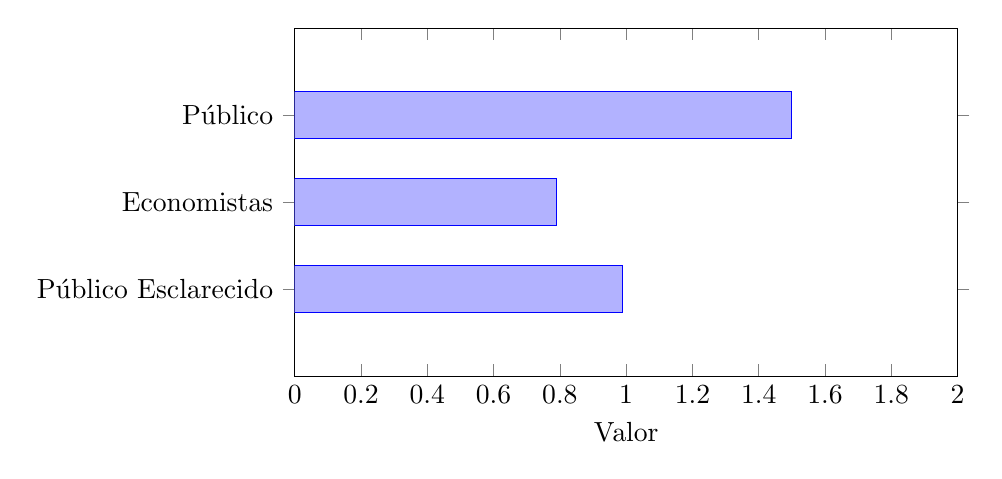
\begin{tikzpicture}
        \begin{axis}[
            xbar,
            symbolic y coords={Público, Economistas, Público Esclarecido},
            ytick=data,
            xmin=0, xmax=2,
            xlabel={Valor},
            bar width=0.6cm,
            width=10cm,
            height=6cm,
            enlarge y limits=0.5,
            y dir=reverse % Invert the y-axis to maintain the desired order
        ]
        \addplot coordinates {(1.5,Público) (0.79,Economistas) (0.99,Público Esclarecido)};
        \end{axis}
    \end{tikzpicture}
    \caption{Elaborado pelo autor com base em Caplan (\citeyear{The_Myth_of_the_Rational_Voter}) \newline
    Nota: As respostas são dadas em uma escala de 0 a 2, onde 0 = “nenhum motivo”, 1 = “motivo menor” e 2 = “motivo principal”.}
    \label{fig:pergunta_1}
\end{figure}


Conforme ilustrado na Figura \ref{fig:pergunta_1}, os economistas demonstram menor preocupação em relação aos problemas advindos da taxação excessiva em comparação ao público em geral. O público mais esclarecido compartilha uma opinião similar, porém ligeiramente mais moderada. Um dos possíveis motivos para essa diferença pode ser que indivíduos com maior riqueza e estabilidade financeira tendem a se preocupar menos com impostos, enquanto aqueles em situações financeiras mais precárias tendem a demonstrar maior preocupação. Este comportamento aparentemente contraria a teoria do viés autoindulgente. A explicação mais plausível para essa discrepância é a influência do viés pessimista, onde as pessoas frequentemente acreditam que são desfavorecidas. Os economistas, entretanto, reconhecem que identificar os "desperdícios" na economia é uma tarefa significativamente mais complexa do que simplesmente atribuir a culpa aos impostos.


\begin{figure}[H]
    \centering
    \caption*{Pergunta 2: “O deficit federal é grande demais”}
    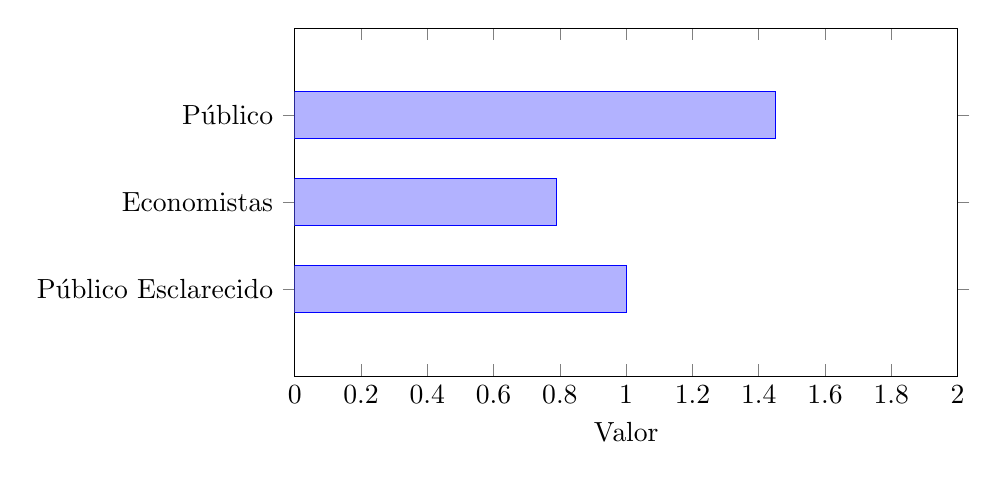
\begin{tikzpicture}
        \begin{axis}[
            xbar,
            symbolic y coords={Público, Economistas, Público Esclarecido},
            ytick=data,
            xmin=0, xmax=2,
            xlabel={Valor},
            bar width=0.6cm,
            width=10cm,
            height=6cm,
            enlarge y limits=0.5,
            y dir=reverse % Invert the y-axis to maintain the desired order
        ]
        \addplot coordinates {(1.45,Público) (0.79,Economistas) (1,Público Esclarecido)};
        \end{axis}
    \end{tikzpicture}
    \caption{Elaborado pelo autor com base em Caplan (\citeyear{The_Myth_of_the_Rational_Voter}) \newline
    Nota: As respostas são dadas em uma escala de 0 a 2, onde 0 = “nenhum motivo”, 1 = “motivo menor” e 2 = “motivo principal”.}
    \label{fig:pergunta_2}
\end{figure}

A Figura \ref{fig:pergunta_2} apresenta uma continuação das opiniões expostas na Figura \ref{fig:pergunta_1}. O público em geral tende a se opor simultaneamente a impostos elevados e a grandes déficits. Em contraste, os economistas demonstram menor preocupação com déficits, enquanto o público esclarecido mantém uma visão mais moderada. A explicação para essa discrepância é consistente com a observada na Figura \ref{fig:pergunta_1}, atribuindo-se ao viés pessimista. Embora os economistas considerem seriamente o problema do déficit federal, eles reconhecem que é uma questão administrável.


\begin{figure}[H]
    \centering
    \caption*{Pergunta 3: “O gasto com ajuda externa é alto demais”}
    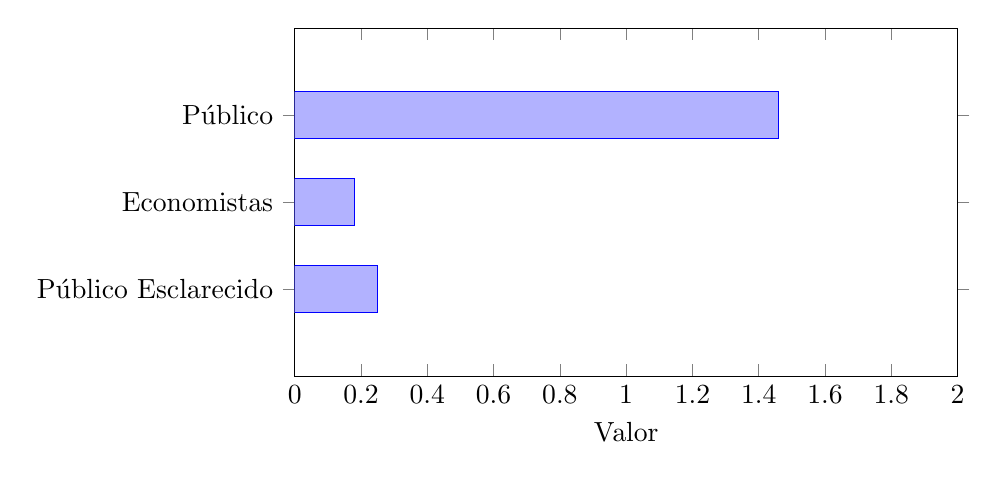
\begin{tikzpicture}
        \begin{axis}[
            xbar,
            symbolic y coords={Público, Economistas, Público Esclarecido},
            ytick=data,
            xmin=0, xmax=2,
            xlabel={Valor},
            bar width=0.6cm,
            width=10cm,
            height=6cm,
            enlarge y limits=0.5,
            y dir=reverse % Invert the y-axis to maintain the desired order
        ]
        \addplot coordinates {(1.46,Público) (0.18,Economistas) (0.25,Público Esclarecido)};
        \end{axis}
    \end{tikzpicture}
    \caption{Elaborado pelo autor com base em Caplan (\citeyear{The_Myth_of_the_Rational_Voter}) \newline
    Nota: As respostas são dadas em uma escala de 0 a 2, onde 0 = “nenhum motivo”, 1 = “motivo menor” e 2 = “motivo principal”.}
    \label{fig:pergunta_3}
\end{figure}

A discrepância de crenças entre o público em geral e os economistas é ainda mais pronunciada na Figura \ref{fig:pergunta_3}. O público em geral tende a acreditar que os gastos com ajuda externa são excessivos, enquanto os economistas discordam dessa percepção. O público esclarecido, por sua vez, possui uma opinião mais alinhada à dos economistas. Para o público em geral, os gastos com ajuda externa constituem um problema significativo, ao passo que os economistas, com o apoio do público esclarecido, não veem esses gastos como um problema tão grave. Existe uma distinção importante entre o financiamento de políticas ineficazes em outros países e a crença de que tais gastos estão levando os Estados Unidos à falência, sendo esta última a opinião predominante no público em geral.

Além disso, não é difícil imaginar a presença do viés antiestrangeiro nessa questão. Uma vez identificados os "bodes-expiatórios" para os problemas internos, torna-se fácil acreditar que os gastos com ajuda externa representam um problema significativo, sem procurar a verdadeira causa dos problemas internos.

\begin{figure}[H]
    \centering
    \caption*{Pergunta 4: “Temos imigrantes demais”}
    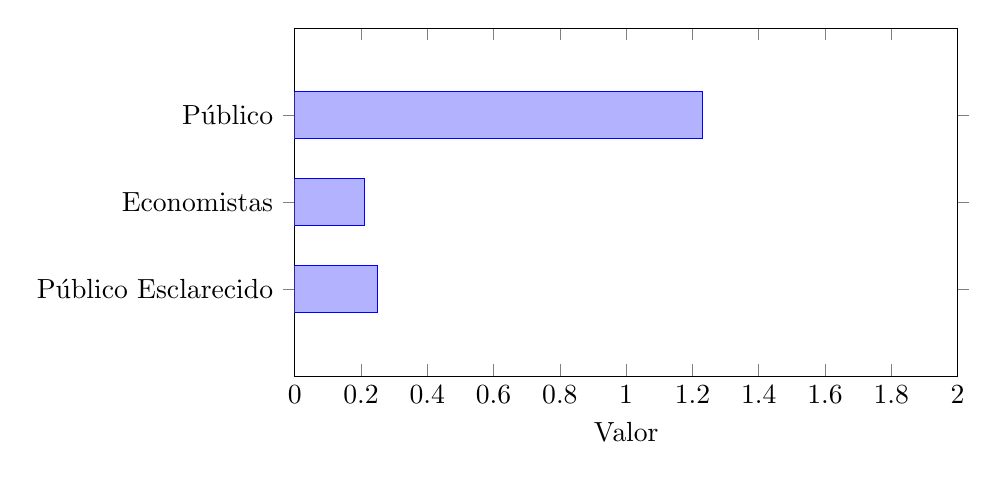
\begin{tikzpicture}
        \begin{axis}[
            xbar,
            symbolic y coords={Público, Economistas, Público Esclarecido},
            ytick=data,
            xmin=0, xmax=2,
            xlabel={Valor},
            bar width=0.6cm,
            width=10cm,
            height=6cm,
            enlarge y limits=0.5,
            y dir=reverse % Invert the y-axis to maintain the desired order
        ]
        \addplot coordinates {(1.23,Público) (0.21,Economistas) (0.25,Público Esclarecido)};
        \end{axis}
    \end{tikzpicture}
    \caption{Elaborado pelo autor com base em Caplan (\citeyear{The_Myth_of_the_Rational_Voter}) \newline
    Nota: As respostas são dadas em uma escala de 0 a 2, onde 0 = “nenhum motivo”, 1 = “motivo menor” e 2 = “motivo principal”.}
    \label{fig:pergunta_4}
\end{figure}

Para quem é afetado pelo viés antiestrangeiro, a questão da imigração é particularmente relevante e até mesmo assustadora. A Figura \ref{fig:pergunta_4} mostra que o público em geral acredita que há muitos imigrantes nos Estados Unidos, enquanto os economistas discordam dessa percepção. O público esclarecido, por sua vez, compartilha a opinião dos economistas. Os economistas reconhecem, ao contrário do público em geral, que um trabalhador independente a mais gera um benefício liquido, independentemente de sua origem. 

Mas por que o público em geral acredita que há muitos imigrantes nos Estados Unidos? A maioria dos medos podem ser um exagero, porém não se tem uma quantidade fixa de postos de trabalho, onde se costumava absorver muito mais novatos nos postos de trabalho, hoje já não se absorve mais. Estudos empíricos no entanto mostram que a imigração não tem um impacto significativo no emprego e nos salários dos trabalhadores nativos \cite{economics-immigration}.





\begin{figure}[H]
    \centering
    \caption*{Pergunta 5: “Há deduções demais para as empresas”}
    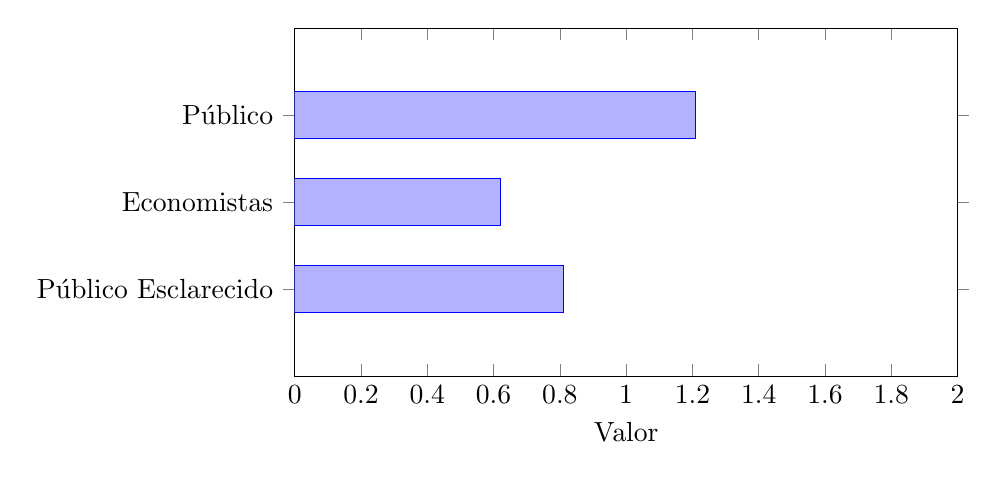
\begin{tikzpicture}
        \begin{axis}[
            xbar,
            symbolic y coords={Público, Economistas, Público Esclarecido},
            ytick=data,
            xmin=0, xmax=2,
            xlabel={Valor},
            bar width=0.6cm,
            width=10cm,
            height=6cm,
            enlarge y limits=0.5,
            y dir=reverse % Invert the y-axis to maintain the desired order
        ]
        \addplot coordinates {(1.21,Público) (0.62,Economistas) (0.81,Público Esclarecido)};
        \end{axis}
    \end{tikzpicture}
    \caption{Elaborado pelo autor com base em Caplan (\citeyear{The_Myth_of_the_Rational_Voter}) \newline
    Nota: As respostas são dadas em uma escala de 0 a 2, onde 0 = “nenhum motivo”, 1 = “motivo menor” e 2 = “motivo principal”.}
    \label{fig:pergunta_5}
\end{figure}


A questão apresentada na figura \ref{fig:pergunta_5} aborda principalmente o viés antimercado. A Pergunta 5: “Há deduções demais para as empresas” refere-se ao excesso de benefícios fiscais concedidos às empresas. A opinião pública considera que os impostos são excessivamente elevados, exceto quando aplicados a empresas gananciosas, que supostamente não estão pagando sua parte justa e, consequentemente, prejudicando a economia. Por outro lado, os economistas têm uma perspectiva distinta, com a qual o público esclarecido tende a concordar.

Ao analisar os fatos, em vez de julgar as empresas com base em uma suposta ganância, diversas fragilidades na visão popular se tornam evidentes. A principal delas é que os incentivos fiscais para as empresas são relativamente pequenos em comparação ao orçamento total. Outro aspecto importante é que os economistas compreendem que a renda corporativa já é sujeita a dupla tributação. Incentivos fiscais ou "brechas" ajudam a atenuar parcialmente as ineficiências decorrentes dessa dupla tributação.

Além disso, o público geralmente desconsidera as complexidades relacionadas à incidência tributária. Em última análise, os consumidores ou trabalhadores podem acabar arcando com o ônus tributário atribuído às empresas. Portanto, enquanto a visão popular é impulsionada por um viés antimercado, uma análise mais aprofundada revela que os incentivos fiscais desempenham um papel mais complexo e menos prejudicial do que se imagina \cite{The_Myth_of_the_Rational_Voter}.





\begin{figure}[H]
    \centering
    \caption*{Pergunta 6: “A educação e a qualificação profissional são inadequadas”}
    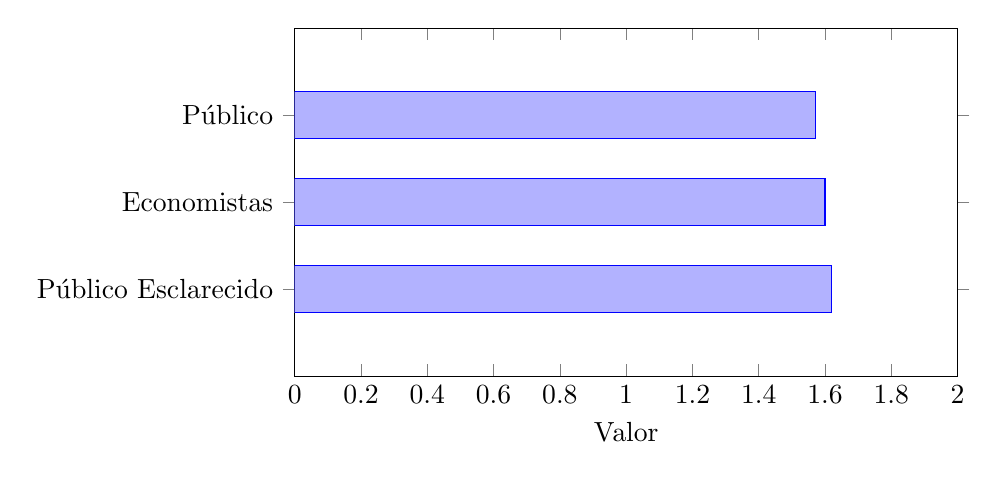
\begin{tikzpicture}
        \begin{axis}[
            xbar,
            symbolic y coords={Público, Economistas, Público Esclarecido},
            ytick=data,
            xmin=0, xmax=2,
            xlabel={Valor},
            bar width=0.6cm,
            width=10cm,
            height=6cm,
            enlarge y limits=0.5,
            y dir=reverse % Invert the y-axis to maintain the desired order
        ]
        \addplot coordinates {(1.57,Público) (1.60,Economistas) (1.62,Público Esclarecido)};
        \end{axis}
    \end{tikzpicture}
    \caption{Elaborado pelo autor com base em Caplan (\citeyear{The_Myth_of_the_Rational_Voter}) \newline
    Nota: As respostas são dadas em uma escala de 0 a 2, onde 0 = “nenhum motivo”, 1 = “motivo menor” e 2 = “motivo principal”.}
    \label{fig:pergunta_6}
\end{figure}

Aqui temos um grande consenso entre o público em geral, os economistas e o público esclarecido. A Figura \ref{fig:pergunta_6} mostra que todos os grupos acreditam que a educação e a qualificação profissional são inadequadas. Os economistas sempre veem a educação como um grande problema a ser superado. O raciocínio é que a educação tem externalidade positiva, fazendo com que o nível de produção do mercado seja menor do que o ótimo. Mesmo sem uma compreensão aprofundada dos mecanismos de externalidades positivas, o público geral reconhece a importância fundamental da educação para o desenvolvimento econômico sustentável.







\begin{figure}[H]
    \centering
    \caption*{Pergunta 7: “A seguridade social atende pessoas demais”}
    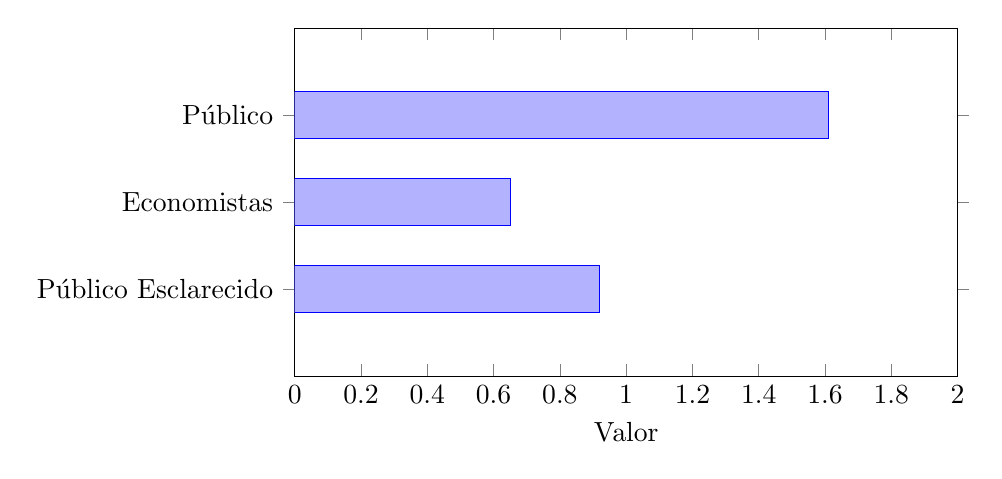
\begin{tikzpicture}
        \begin{axis}[
            xbar,
            symbolic y coords={Público, Economistas, Público Esclarecido},
            ytick=data,
            xmin=0, xmax=2,
            xlabel={Valor},
            bar width=0.6cm,
            width=10cm,
            height=6cm,
            enlarge y limits=0.5,
            y dir=reverse % Invert the y-axis to maintain the desired order
        ]
        \addplot coordinates {(1.61,Público) (0.65,Economistas) (0.92,Público Esclarecido)};
        \end{axis}
    \end{tikzpicture}
    \caption{Elaborado pelo autor com base em Caplan (\citeyear{The_Myth_of_the_Rational_Voter}) \newline
    Nota: As respostas são dadas em uma escala de 0 a 2, onde 0 = “nenhum motivo”, 1 = “motivo menor” e 2 = “motivo principal”.}
    \label{fig:pergunta_7}
\end{figure}

Novamente, os economistas desafiam sua reputação conservadora. Embora frequentemente apontem os efeitos ocultos de desincentivo dos programas governamentais, o público já está acostumado com a ideia de que, ao ajudar os pobres, eles se tornam menos propensos a se ajudarem \cite{Murray1985-MURLGA-3}. A disputa reside na magnitude desses efeitos. Influenciados por seu viés pessimista, os não economistas tendem a superestimar o impacto negativo dos desincentivos do bem-estar social.

Onde o público erra? Principalmente na interpretação da relevância dos números. Os programas de combate à pobreza, mesmo quando amplamente considerados, correspondem a uma fração relativamente pequena dos gastos governamentais. Embora essa fração seja significativamente maior do que a destinada à ajuda externa, ainda é insuficiente para ser vista como uma causa principal para o desempenho econômico abaixo do esperado. Além disso, os beneficiários do bem-estar social geralmente pertencem ao segmento menos qualificado da população, o que limita o impacto econômico de sua ausência no mercado de trabalho.



\begin{figure}[H]
    \centering
    \caption*{Pergunta 8: “Mulheres e minorias tem vantagens demais por causa das ações afirmativas”}
    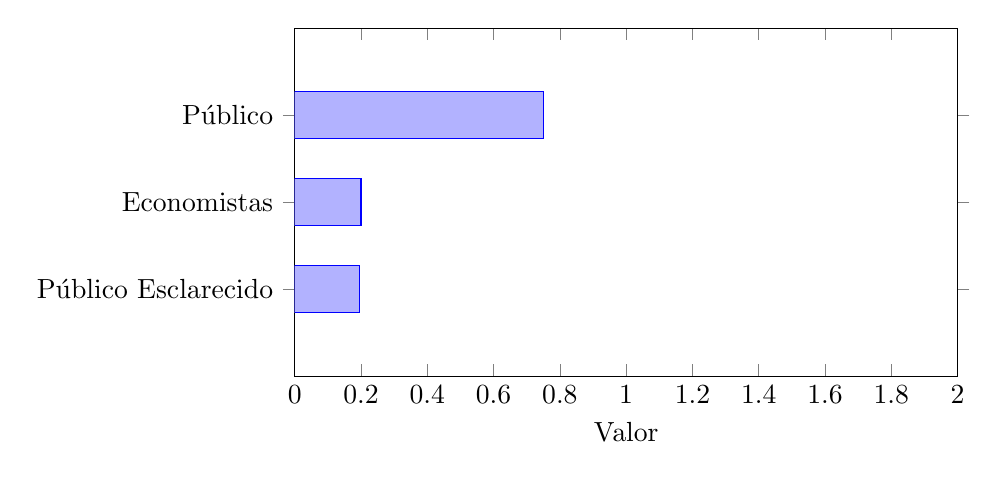
\begin{tikzpicture}
        \begin{axis}[
            xbar,
            symbolic y coords={Público, Economistas, Público Esclarecido},
            ytick=data,
            xmin=0, xmax=2,
            xlabel={Valor},
            bar width=0.6cm,
            width=10cm,
            height=6cm,
            enlarge y limits=0.5,
            y dir=reverse % Invert the y-axis to maintain the desired order
        ]
        \addplot coordinates {(0.75,Público) (0.2,Economistas) (0.195,Público Esclarecido)};
        \end{axis}
    \end{tikzpicture}
    \caption{Elaborado pelo autor com base em Caplan (\citeyear{The_Myth_of_the_Rational_Voter}) \newline
    Nota: As respostas são dadas em uma escala de 0 a 2, onde 0 = “nenhum motivo”, 1 = “motivo menor” e 2 = “motivo principal”.}
    \label{fig:pergunta_8}
\end{figure}


Ações afirmativas são estudadas a tempos e seus efeitos conhecidos \cite{sowell2004affirmative}. Dar a categorias especiais de empregados o direito de processar os seus empregadores torna-os menos propensos a serem contratados. Mas os economistas, no entanto, atribuem ao problema menos importância global do que o público. A razão é provavelmente quantitativa: apesar do pessimismo do público, há muito poucos processos judiciais por discriminação para serem mais do que um problema menor \cite{The_Myth_of_the_Rational_Voter}.




\begin{figure}[H]
    \centering
    \caption*{Pergunta 9: “As pessoas não dão valor ao trabalho duro”}
    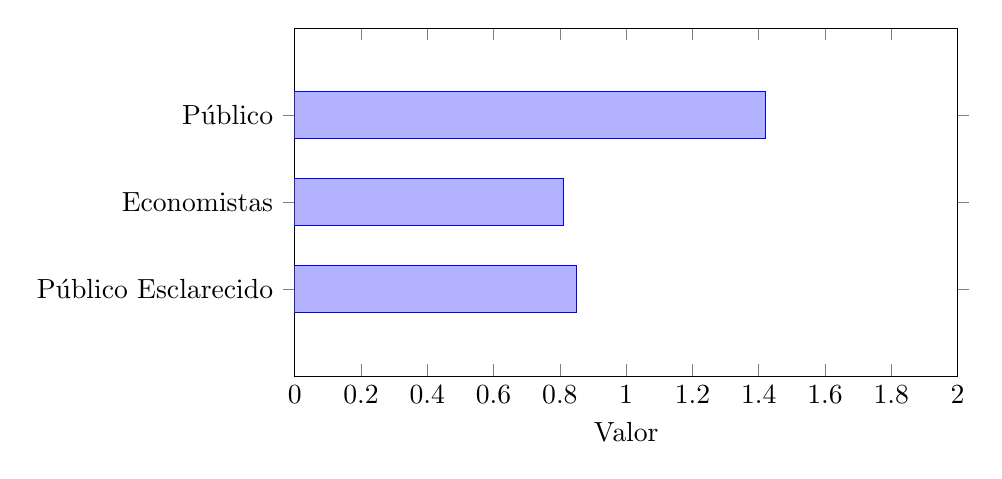
\begin{tikzpicture}
        \begin{axis}[
            xbar,
            symbolic y coords={Público, Economistas, Público Esclarecido},
            ytick=data,
            xmin=0, xmax=2,
            xlabel={Valor},
            bar width=0.6cm,
            width=10cm,
            height=6cm,
            enlarge y limits=0.5,
            y dir=reverse % Invert the y-axis to maintain the desired order
        ]
        \addplot coordinates {(1.42,Público) (0.81,Economistas) (0.85,Público Esclarecido)};
        \end{axis}
    \end{tikzpicture}
    \caption{Elaborado pelo autor com base em Caplan (\citeyear{The_Myth_of_the_Rational_Voter}) \newline
    Nota: As respostas são dadas em uma escala de 0 a 2, onde 0 = “nenhum motivo”, 1 = “motivo menor” e 2 = “motivo principal”.}
    \label{fig:pergunta_9}
\end{figure}

Aqui pode-se ter uma ideia dos leigos com o viés pessimista. A visão de uma sociedade em decadência por causa da virtude em colapso é observada. Para os economistas por outro lado, a virtude é um problema menor, fazendo parte dos sintomas do progresso e não sendo uma declaração de decadência. Novamente o público esclarecido se alinha com os economistas. 













\begin{figure}[H]
    \centering
    \caption*{Pergunta 10: “O governo regulamenta muito os negócios”}
    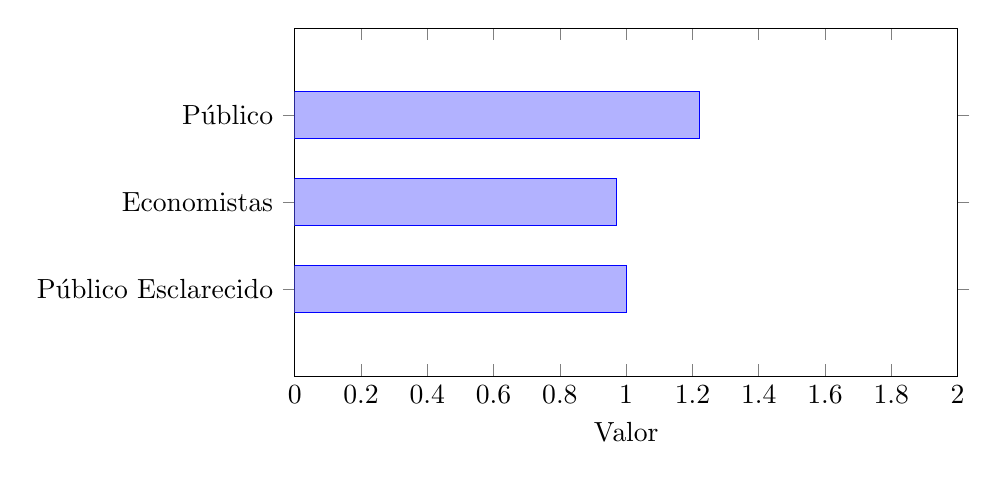
\begin{tikzpicture}
        \begin{axis}[
            xbar,
            symbolic y coords={Público, Economistas, Público Esclarecido},
            ytick=data,
            xmin=0, xmax=2,
            xlabel={Valor},
            bar width=0.6cm,
            width=10cm,
            height=6cm,
            enlarge y limits=0.5,
            y dir=reverse % Invert the y-axis to maintain the desired order
        ]
        \addplot coordinates {(1.22,Público) (0.97,Economistas) (1,Público Esclarecido)};
        \end{axis}
    \end{tikzpicture}
    \caption{Elaborado pelo autor com base em Caplan (\citeyear{The_Myth_of_the_Rational_Voter}) \newline
    Nota: As respostas são dadas em uma escala de 0 a 2, onde 0 = “nenhum motivo”, 1 = “motivo menor” e 2 = “motivo principal”.}
    \label{fig:pergunta_10}
\end{figure}

A percepção de que os economistas são desregulamentadores dogmáticos parece ser exagerada nesta questão. Eles tendem a considerar os problemas de regulamentação como menos graves em comparação ao público geral, que frequentemente adota uma visão mais pessimista.

Embora essa postura possa ser vista como uma evidência contrária ao viés antimercado, há indícios que atenuam essa interpretação. A população em geral apoia consistentemente a regulamentação em áreas específicas, como segurança alimentar e proteção ambiental, conforme evidenciado por pesquisas de opinião que mantêm essa tendência ao longo do tempo \cite{pew_research_2023}. Para o público, os principais custos da regulamentação incluem burocracia, ineficiência e proibições. Em contrapartida, os economistas geralmente argumentam que a regulamentação é contraproducente e prejudicial à economia a longo prazo. Além disso, há ceticismo quanto aos verdadeiros objetivos da regulamentação, questionando se visa proteger o consumidor ou servir aos interesses de grupos específicos \cite{rowley1988political, weiss1986regulatory,The_Myth_of_the_Rational_Voter}.







\begin{figure}[H]
    \centering
    \caption*{Pergunta 11: “As pessoas não poupão o bastante”}
    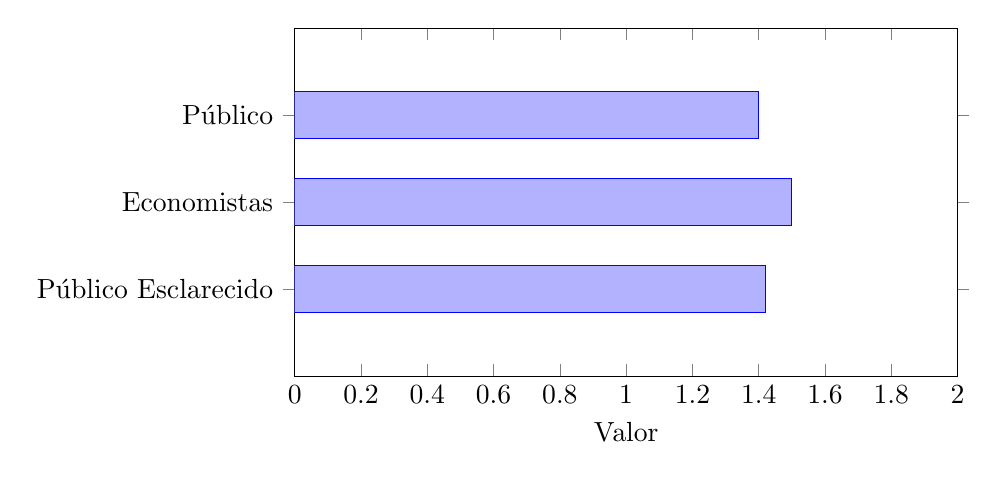
\begin{tikzpicture}
        \begin{axis}[
            xbar,
            symbolic y coords={Público, Economistas, Público Esclarecido},
            ytick=data,
            xmin=0, xmax=2,
            xlabel={Valor},
            bar width=0.6cm,
            width=10cm,
            height=6cm,
            enlarge y limits=0.5,
            y dir=reverse % Invert the y-axis to maintain the desired order
        ]
        \addplot coordinates {(1.4,Público) (1.5,Economistas) (1.42,Público Esclarecido)};
        \end{axis}
    \end{tikzpicture}
    \caption{Elaborado pelo autor com base em Caplan (\citeyear{The_Myth_of_the_Rational_Voter}) \newline
    Nota: As respostas são dadas em uma escala de 0 a 2, onde 0 = “nenhum motivo”, 1 = “motivo menor” e 2 = “motivo principal”.}
    \label{fig:pergunta_11}
\end{figure}

Leigos e especialistas estão quase igualmente preocupados com a baixa taxa de poupança como observado na figura \ref{fig:pergunta_11}. O medo é a posição padrão do público; este é um caso raro em que os economistas concordam. Existem duas razões principais para o alto nível de preocupação dos especialistas. Primeiro, a poupança é tributada duas vezes. Paga-se um imposto quando se ganha renda e um imposto adicional se houver rendimento sobre a renda após o imposto. Isso sugere uma diferença incomumente grande entre o nível eficiente de poupança, sem impostos, e o nível real. Segundo, muitos economistas acreditam que a poupança possui externalidades positivas, portanto, mesmo sem impostos, o nível de poupança ainda seria insuficiente \cite{The_Myth_of_the_Rational_Voter}.

\subsubsection{Por que a economia não está crescendo? - Parte 2}

O enunciado para as próximas sete perguntas do SAEE muda ligeiramente: "Agora vou ler para você outra lista de razões, relacionadas aos negócios, que algumas pessoas deram para explicar por que a economia não está melhor do que está. Para cada uma, por favor, me diga se você acha que é um motivo principal pela qual a economia não está melhor do que está, um motivo menor ou não é uma razão de forma alguma." \cite{saee1996}.

\begin{figure}[H]
    \centering
    \caption*{Pergunta 12: “As empresas lucram demais”}
    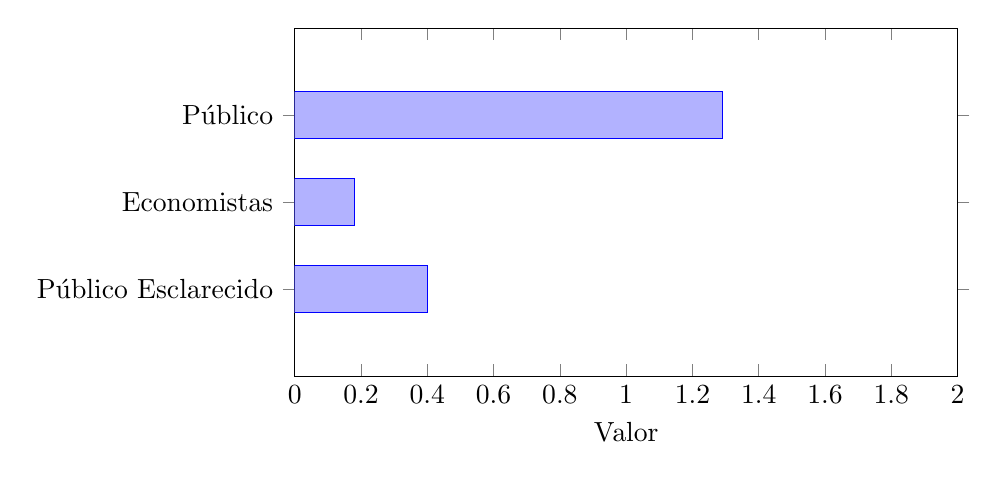
\begin{tikzpicture}
        \begin{axis}[
            xbar,
            symbolic y coords={Público, Economistas, Público Esclarecido},
            ytick=data,
            xmin=0, xmax=2,
            xlabel={Valor},
            bar width=0.6cm,
            width=10cm,
            height=6cm,
            enlarge y limits=0.5,
            y dir=reverse % Invert the y-axis to maintain the desired order
        ]
        \addplot coordinates {(1.29,Público) (0.18,Economistas) (0.4,Público Esclarecido)};
        \end{axis}
    \end{tikzpicture}
    \caption{Elaborado pelo autor com base em Caplan (\citeyear{The_Myth_of_the_Rational_Voter}) \newline
    Nota: As respostas são dadas em uma escala de 0 a 2, onde 0 = “nenhum motivo”, 1 = “motivo menor” e 2 = “motivo principal”.}
    \label{fig:pergunta_12}
\end{figure}

A presente análise fornece mais uma evidência contrária à ideia do viés autoindulgente. Economistas rejeitam a noção de que lucros excessivos prejudicam a economia. E não dizem isso por serem os "malfeitores riquinhos". Na verdade, os dados mostram que, independentemente de sua condição econômica, economistas com PhD compartilham essa visão \cite{The_Myth_of_the_Rational_Voter}.

O verdadeiro problema reside no fato de que o público em geral não compreende o papel dos lucros na economia, sendo o viés antimercado um dos principais responsáveis por essa miopia. Enquanto o público geralmente vê o lucro como uma transferência de renda dos pobres para os ricos, os economistas o veem como um sinal de eficiência e um motor de progresso e flexibilidade econômica.

\begin{figure}[H]
    \centering
    \caption*{Pergunta 13: “Altos executivos ganham demais”}
    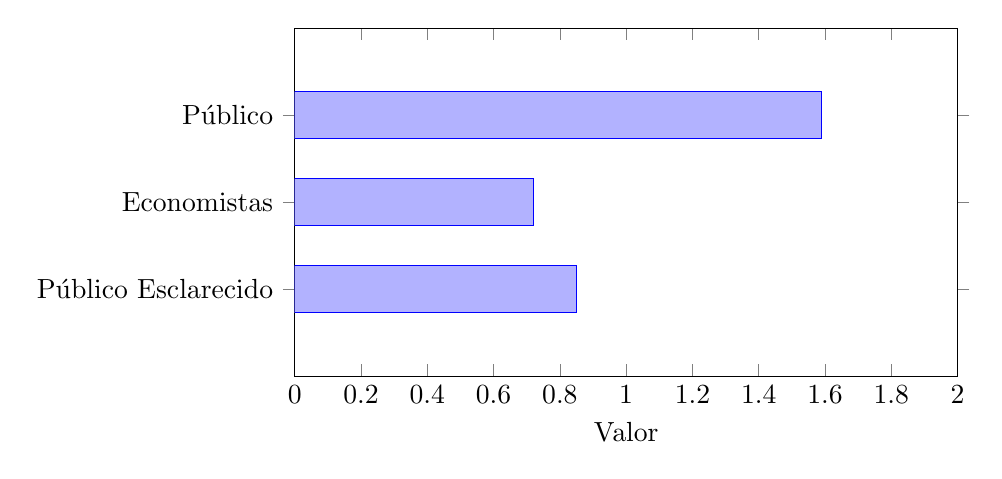
\begin{tikzpicture}
        \begin{axis}[
            xbar,
            symbolic y coords={Público, Economistas, Público Esclarecido},
            ytick=data,
            xmin=0, xmax=2,
            xlabel={Valor},
            bar width=0.6cm,
            width=10cm,
            height=6cm,
            enlarge y limits=0.5,
            y dir=reverse % Invert the y-axis to maintain the desired order
        ]
        \addplot coordinates {(1.59,Público) (0.72,Economistas) (0.85,Público Esclarecido)};
        \end{axis}
    \end{tikzpicture}
    \caption{Elaborado pelo autor com base em Caplan (\citeyear{The_Myth_of_the_Rational_Voter}) \newline
    Nota: As respostas são dadas em uma escala de 0 a 2, onde 0 = “nenhum motivo”, 1 = “motivo menor” e 2 = “motivo principal”.}
    \label{fig:pergunta_13}
\end{figure}

As crenças sobre remuneração executiva excessiva são semelhantes às crenças sobre lucros excessivos. Os números do Público Esclarecido se alinham com a narrativa de que "os especialistas estão certos, os leigos estão errados". Mais uma vez, devemos deixar de nos preocupar com o viés autoindulgente dos economistas e começar a nos preocupar com o viés antimercado dos não economistas. Para o público em geral, a remuneração dos executivos é vista como uma transferência para os gestores de alto nível: quando eles ganham mais, os subordinados ganham menos. Os economistas rejeitam essa mentalidade de soma zero. Eles argumentam que os salários dos capitães da indústria fornecem incentivos para reduzir custos, criar e melhorar produtos e prever com precisão a demanda dos consumidores.

Os economistas estão mais inclinados a considerar a possibilidade de que a compensação executiva não está suficientemente atrelada ao desempenho. Portanto, embora a remuneração elevada não seja, por si só, um problema, a remuneração excessivamente alta, quando não associada ao desempenho, pode ser problemática. A questão é mais complexa do que a visão popular sugere, e a solução não é simplesmente limitar a remuneração dos executivos \cite{The_Myth_of_the_Rational_Voter}.



\begin{figure}[H]
    \centering
    \caption*{Pergunta 14: “A produtividade está aumentando devagar demais”}
    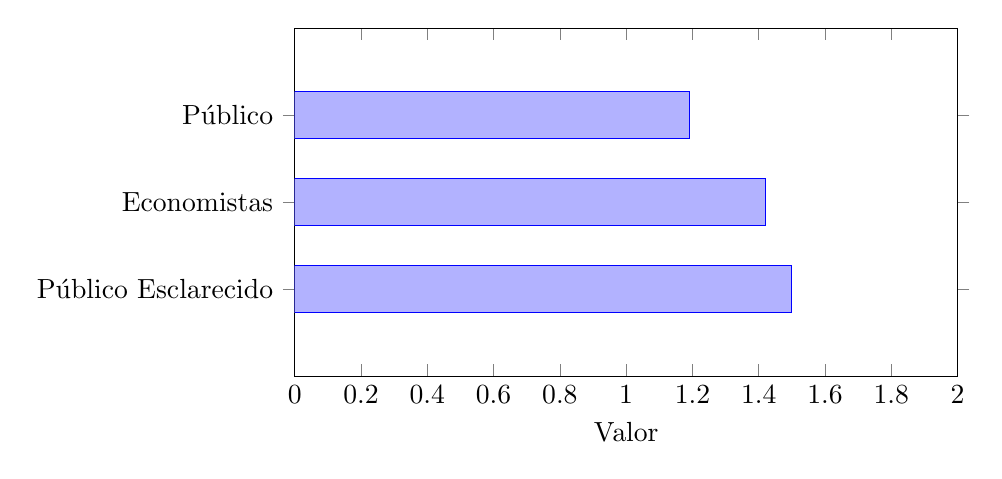
\begin{tikzpicture}
        \begin{axis}[
            xbar,
            symbolic y coords={Público, Economistas, Público Esclarecido},
            ytick=data,
            xmin=0, xmax=2,
            xlabel={Valor},
            bar width=0.6cm,
            width=10cm,
            height=6cm,
            enlarge y limits=0.5,
            y dir=reverse % Invert the y-axis to maintain the desired order
        ]
        \addplot coordinates {(1.19,Público) (1.42,Economistas) (1.5,Público Esclarecido)};
        \end{axis}
    \end{tikzpicture}
    \caption{Elaborado pelo autor com base em Caplan (\citeyear{The_Myth_of_the_Rational_Voter}) \newline
    Nota: As respostas são dadas em uma escala de 0 a 2, onde 0 = “nenhum motivo”, 1 = “motivo menor” e 2 = “motivo principal”.}
    \label{fig:pergunta_14}
\end{figure}

A produtividade empresarial é o único problema que claramente preocupa os economistas mais do que o público geral, embora seja possível argumentar que essa divergência é semântica. O termo “produtividade empresarial” pode parecer vagamente desejável para os leigos. No entanto, para os economistas, possui um significado preciso: refere-se à parte da produção que não pode ser atribuída ao trabalho ou ao capital. Intuitivamente, o crescimento da produtividade empresarial indica que os mesmos insumos resultam em um maior output. Caso os não-economistas compreendessem a terminologia econômica, talvez suas avaliações se alinhassem mais com as dos economistas.

\begin{figure}[H]
    \centering
    \caption*{Pergunta 15: “A tecnologia causa demissões”}
    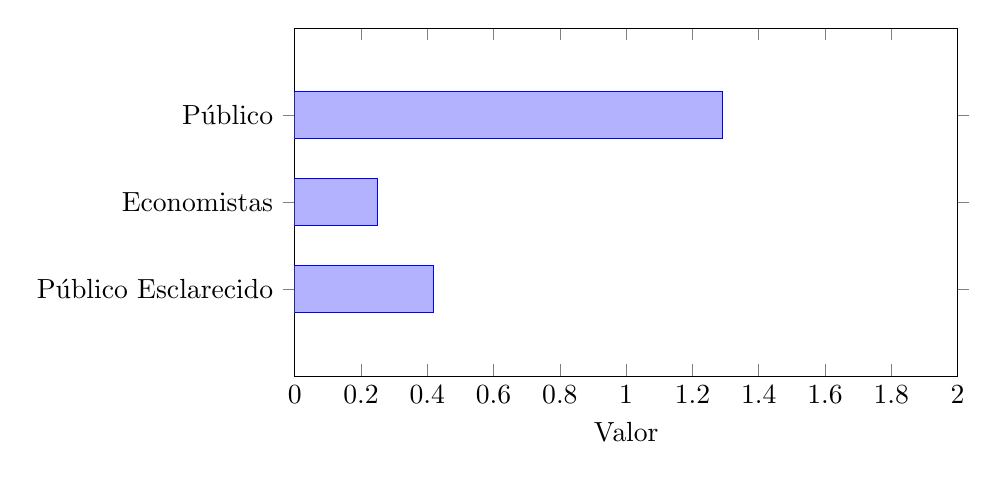
\begin{tikzpicture}
        \begin{axis}[
            xbar,
            symbolic y coords={Público, Economistas, Público Esclarecido},
            ytick=data,
            xmin=0, xmax=2,
            xlabel={Valor},
            bar width=0.6cm,
            width=10cm,
            height=6cm,
            enlarge y limits=0.5,
            y dir=reverse % Invert the y-axis to maintain the desired order
        ]
        \addplot coordinates {(1.29,Público) (0.25,Economistas) (0.42,Público Esclarecido)};
        \end{axis}
    \end{tikzpicture}
    \caption{Elaborado pelo autor com base em Caplan (\citeyear{The_Myth_of_the_Rational_Voter}) \newline
    Nota: As respostas são dadas em uma escala de 0 a 2, onde 0 = “nenhum motivo”, 1 = “motivo menor” e 2 = “motivo principal”.}
    \label{fig:pergunta_15}
\end{figure}

É evidente que as máquinas contribuem significativamente para o aumento da riqueza. A tecnologia representa uma das diferenças mais notórias entre o presente e o passado, bem como entre o Primeiro Mundo e o Terceiro Mundo. No entanto, os dados mostram que muitos adotam um viés de "trabalho forçado" em sua forma mais crua: o medo da máquina. De fato, é provável que haja um ressentimento em relação àqueles que não compartilham desse medo, especialmente economistas acadêmicos que não “sentem a dor” do trabalhador sem estabilidade. No entanto, essa acusação se revela infundada; o Público esclarecido adota a posição "extrema" dos economistas com apenas uma leve moderação \cite{The_Myth_of_the_Rational_Voter}. 

\begin{figure}[H]
    \centering
    \caption*{Pergunta 16: “As empresas estão enviando funcionários ao estrangeiro”}
    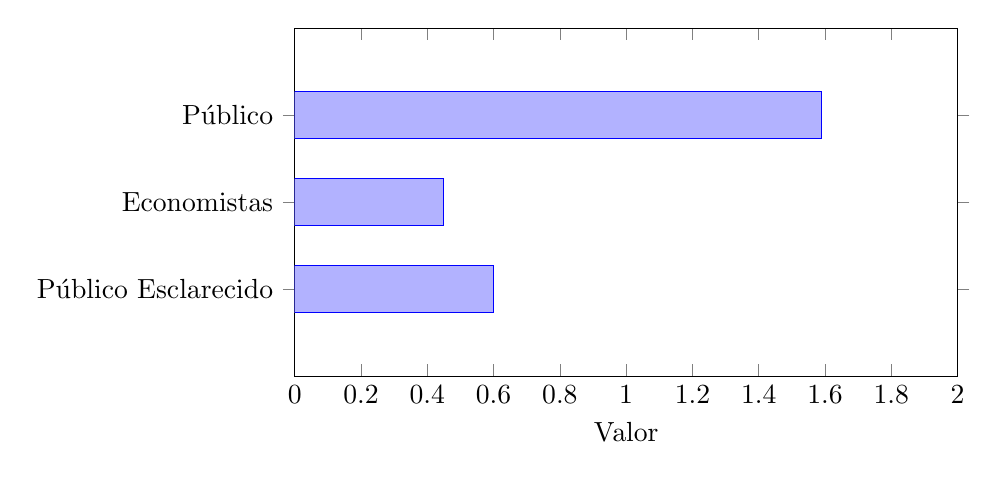
\begin{tikzpicture}
        \begin{axis}[
            xbar,
            symbolic y coords={Público, Economistas, Público Esclarecido},
            ytick=data,
            xmin=0, xmax=2,
            xlabel={Valor},
            bar width=0.6cm,
            width=10cm,
            height=6cm,
            enlarge y limits=0.5,
            y dir=reverse % Invert the y-axis to maintain the desired order
        ]
        \addplot coordinates {(1.59,Público) (0.45,Economistas) (0.6,Público Esclarecido)};
        \end{axis}
    \end{tikzpicture}
    \caption{Elaborado pelo autor com base em Caplan (\citeyear{The_Myth_of_the_Rational_Voter}) \newline
    Nota: As respostas são dadas em uma escala de 0 a 2, onde 0 = “nenhum motivo”, 1 = “motivo menor” e 2 = “motivo principal”.}
    \label{fig:pergunta_16}
\end{figure}

Se economistas e o público concordassem quanto aos perigos econômicos de "enviar empregos para o exterior", a alegação de que o público sofre de viés antiestrangeiro teria que ser reconsiderada. Na realidade, essa é a segunda maior disparidade na SAEE, superada apenas pela diferença de crenças sobre ajuda externa. O desprezo dos economistas pelo problema da ajuda externa decorre de seu conhecimento sobre o orçamento. Se os Estados Unidos gastassem extremamente mais em ajuda externa, os economistas reconheceriam que isso representaria um grande ônus para o padrão de vida dos americanos. A falta de preocupação com a transferência de empregos para o exterior é mais fundamentada na teoria. De acordo com a Lei das Vantagens Comparativas, os empregos "vão para o exterior" porque há maneiras mais remuneradoras de utilizar o trabalho doméstico \cite{krugman2015accidental,blinder1987hard}.



\begin{figure}[H]
    \centering
    \caption*{Pergunta 17: “As empresas estão reduzindo os postos de trabalho”}
    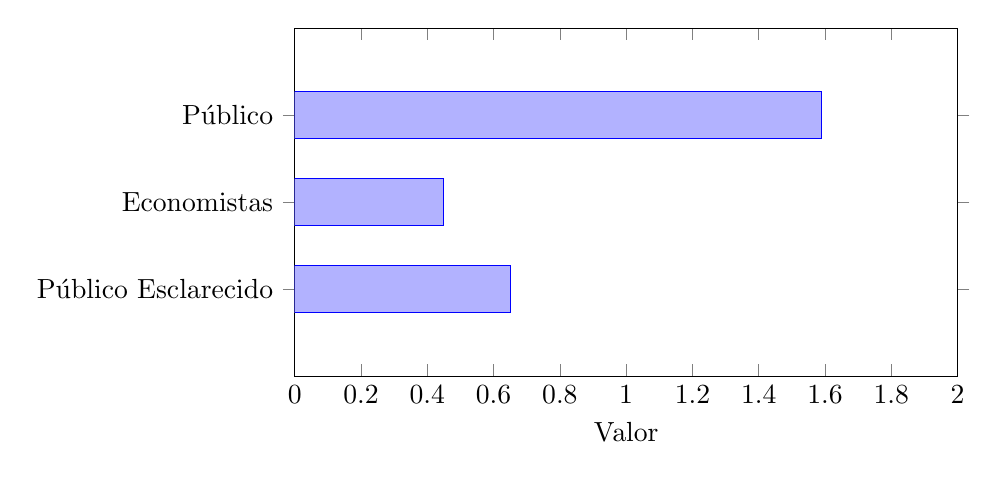
\begin{tikzpicture}
        \begin{axis}[
            xbar,
            symbolic y coords={Público, Economistas, Público Esclarecido},
            ytick=data,
            xmin=0, xmax=2,
            xlabel={Valor},
            bar width=0.6cm,
            width=10cm,
            height=6cm,
            enlarge y limits=0.5,
            y dir=reverse % Invert the y-axis to maintain the desired order
        ]
        \addplot coordinates {(1.59,Público) (0.45,Economistas) (0.65,Público Esclarecido)};
        \end{axis}
    \end{tikzpicture}
    \caption{Elaborado pelo autor com base em Caplan (\citeyear{The_Myth_of_the_Rational_Voter}) \newline
    Nota: As respostas são dadas em uma escala de 0 a 2, onde 0 = “nenhum motivo”, 1 = “motivo menor” e 2 = “motivo principal”.}
    \label{fig:pergunta_17}
\end{figure}

Quando uma empresa lucrativa reduz sua força de trabalho, a percepção comum é de que isso é claramente prejudicial para a economia. A redução é considerada aceitável se uma empresa demite trabalhadores para evitar a falência, sacrificando alguns empregos para preservar outros. No entanto, uma empresa lucrativa que realiza cortes para se tornar ainda mais lucrativa é amplamente condenada. Isso ocorre principalmente entre aqueles que sofrem de viés antitrabalho. A visão popular baseia-se na ilusão de que o emprego, e não a produção, é a verdadeira medida da prosperidade. Em contraste, para economistas e para o Público Iluminado, a redução de pessoal confirma a regra de que o interesse privado e o interesse público podem seguir na mesma direção \cite{Myths-of-Rich-and-Poor,The_Myth_of_the_Rational_Voter}. A redução de trabalhadores excedentes leva esses indivíduos a buscar formas mais socialmente produtivas de aplicar suas habilidades. Imagine se os campos do século XIX nunca tivessem “reduzido” sua força de trabalho. A economia moderna seria muito menos produtiva e muito mais pobre, com a maioria da população trabalhando em fazendas.


\begin{figure}[H]
    \centering
    \caption*{Pergunta 18: “As empresas não investem o suficiente em educação e qualificação profissional”}
    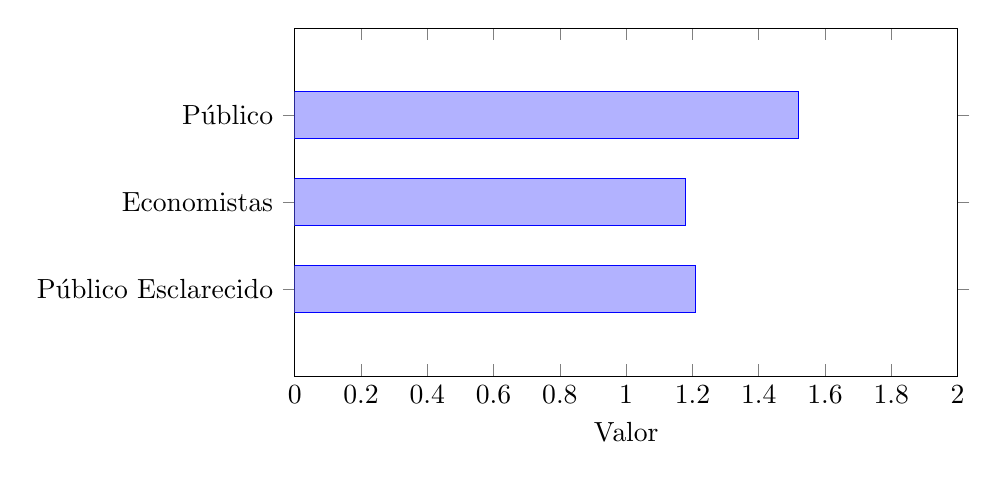
\begin{tikzpicture}
        \begin{axis}[
            xbar,
            symbolic y coords={Público, Economistas, Público Esclarecido},
            ytick=data,
            xmin=0, xmax=2,
            xlabel={Valor},
            bar width=0.6cm,
            width=10cm,
            height=6cm,
            enlarge y limits=0.5,
            y dir=reverse % Invert the y-axis to maintain the desired order
        ]
        \addplot coordinates {(1.52,Público) (1.18,Economistas) (1.21,Público Esclarecido)};
        \end{axis}
    \end{tikzpicture}
    \caption{Elaborado pelo autor com base em Caplan (\citeyear{The_Myth_of_the_Rational_Voter}) \newline
    Nota: As respostas são dadas em uma escala de 0 a 2, onde 0 = “nenhum motivo”, 1 = “motivo menor” e 2 = “motivo principal”.}
    \label{fig:pergunta_18}
\end{figure}

Há um consenso amplo de que a educação inadequada é um problema econômico significativo. O item na pergunta 18 propõe uma hipótese sobre o motivo pelo qual estamos insuficientemente educados: a falta de investimento por parte das empresas. Essa explicação pode atrair indivíduos com viés antimercado, e essa perspectiva parece apropriada: enquanto economistas e o Público Esclarecido não descartam essa explicação, o público em geral demonstra uma simpatia mais pronunciada por ela. 


\subsubsection{Bom, ruim ou neutro para a economia?}

Todas as questões apresentadas anteriormente são sobre o que está impedindo a economia de crescer, ou seja, problemas econômicos. As próximas sete perguntas mais gerais, são sobre se algo é bom, ruim ou neutro para a economia: "Em termos gerais, você acha que as seguintes coisas são boas, ruins ou neutras para a economia?" \cite{saee1996}.

\begin{figure}[H]
    \centering
    \caption*{Pergunta 19: “Corte de impostos”}
    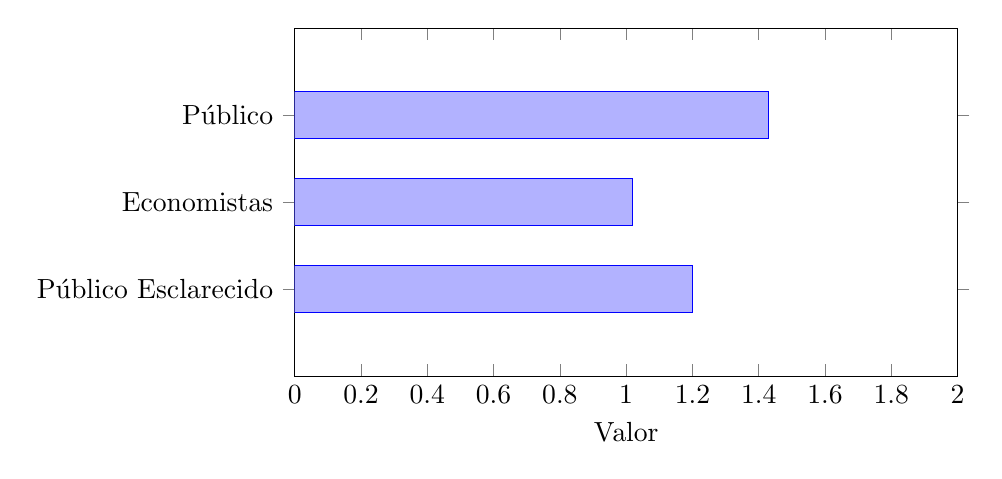
\begin{tikzpicture}
        \begin{axis}[
            xbar,
            symbolic y coords={Público, Economistas, Público Esclarecido},
            ytick=data,
            xmin=0, xmax=2,
            xlabel={Valor},
            bar width=0.6cm,
            width=10cm,
            height=6cm,
            enlarge y limits=0.5,
            y dir=reverse % Invert the y-axis to maintain the desired order
        ]
        \addplot coordinates {(1.43,Público) (1.02,Economistas) (1.2,Público Esclarecido)};
        \end{axis}
    \end{tikzpicture}
    \caption{Elaborado pelo autor com base em Caplan (\citeyear{The_Myth_of_the_Rational_Voter}) \newline
    Nota: As respostas são dadas em uma escala de 0 a 2, onde 0 = “ruim”, 1 = “indiferente” e 2 = “bom”.}
    \label{fig:pergunta_19}
\end{figure}

O público acredita que os impostos são excessivamente altos e, consequentemente, considera que cortes de impostos são uma medida benéfica. A interpretação feita é de que os não-economistas, geralmente pessimistas, estão convencidos de que o governo desperdiça seu dinheiro. Eles, portanto, esperam ingenuamente que os cortes de impostos possam ser financiados através da redução de programas impopulares e do “desperdício”. Em contraste, os economistas, apesar de sua imagem de \textit{laissez-faire}, são céticos. Programas impopulares representam apenas uma pequena fração do orçamento, e o “desperdício” não pode ser identificado de forma inquestionável \cite{krugman2015accidental,The_Myth_of_the_Rational_Voter}.



\begin{figure}[H]
    \centering
    \caption*{Pergunta 20: “Mais mulheres entram para a força de trabalho”}
    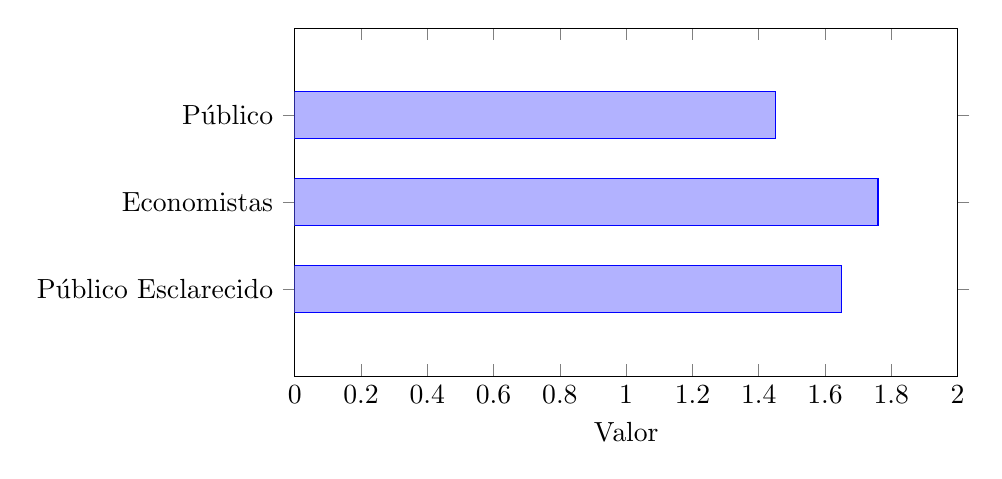
\begin{tikzpicture}
        \begin{axis}[
            xbar,
            symbolic y coords={Público, Economistas, Público Esclarecido},
            ytick=data,
            xmin=0, xmax=2,
            xlabel={Valor},
            bar width=0.6cm,
            width=10cm,
            height=6cm,
            enlarge y limits=0.5,
            y dir=reverse % Invert the y-axis to maintain the desired order
        ]
        \addplot coordinates {(1.45,Público) (1.76,Economistas) (1.65,Público Esclarecido)};
        \end{axis}
    \end{tikzpicture}
    \caption{Elaborado pelo autor com base em Caplan (\citeyear{The_Myth_of_the_Rational_Voter}) \newline
    Nota: As respostas são dadas em uma escala de 0 a 2, onde 0 = “ruim”, 1 = “indiferente” e 2 = “bom”.}
    \label{fig:pergunta_20}
\end{figure}

Economistas e a maioria da população veem o aumento da participação feminina na força de trabalho como um desenvolvimento positivo. No entanto, uma certa reserva pode ser observada entre alguns grupos, que são menos unânimes sobre essa mudança. É interessante notar que há uma percepção otimista em relação ao aumento da oferta de trabalho feminino, enquanto o aumento da oferta de trabalho imigrante frequentemente enfrenta ceticismo, apesar dos efeitos econômicos potenciais de ambos serem semelhantes. Uma possível explicação para essa diferença de percepção pode ser a influência das normas sociais e das preocupações com questões de justiça e igualdade, que podem tornar mais difícil discutir abertamente as implicações econômicas desses aumentos de forma comparativa.


\begin{figure}[H]
    \centering
    \caption*{Pergunta 21: “Aumento do uso de tecnologia no trabalho”}
    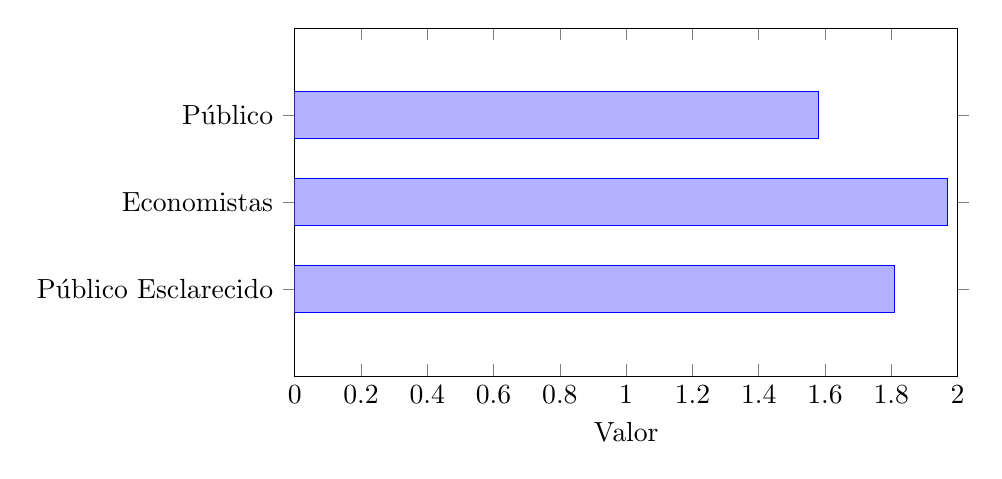
\begin{tikzpicture}
        \begin{axis}[
            xbar,
            symbolic y coords={Público, Economistas, Público Esclarecido},
            ytick=data,
            xmin=0, xmax=2,
            xlabel={Valor},
            bar width=0.6cm,
            width=10cm,
            height=6cm,
            enlarge y limits=0.5,
            y dir=reverse % Invert the y-axis to maintain the desired order
        ]
        \addplot coordinates {(1.58,Público) (1.97,Economistas) (1.81,Público Esclarecido)};
        \end{axis}
    \end{tikzpicture}
    \caption{Elaborado pelo autor com base em Caplan (\citeyear{The_Myth_of_the_Rational_Voter}) \newline
    Nota: As respostas são dadas em uma escala de 0 a 2, onde 0 = “ruim”, 1 = “indiferente” e 2 = “bom”.}
    \label{fig:pergunta_21}
\end{figure}

Apesar de vários preconceitos, a maioria das pessoas reconhece que a tecnologia é benéfica para a economia. A maioria confortável reconhece os benefícios da tecnologia. A lacuna que temos é de que os economistas aceitam a tecnologia a uma só voz, enquanto o público em geral é mais cético. Onde antes os economistas não conseguiam concordar, agora é a vez do público em geral. É muito alta a chance de se ouvir dizer "Sim, a tecnologia é boa para a economia, mas..." \cite{The_Myth_of_the_Rational_Voter}.

\begin{figure}[H]
    \centering
    \caption*{Pergunta 22: “Acordos comerciais entre os Estados Unidos e os outros países”}
    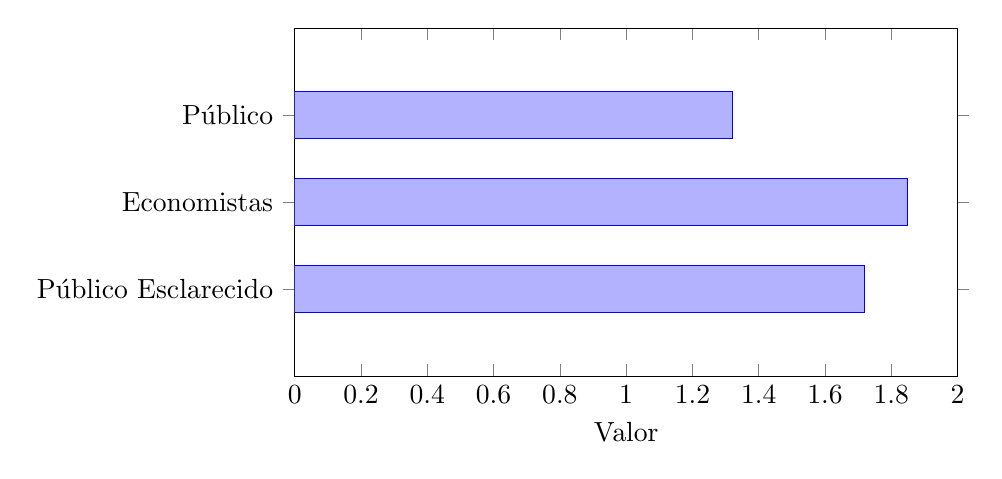
\begin{tikzpicture}
        \begin{axis}[
            xbar,
            symbolic y coords={Público, Economistas, Público Esclarecido},
            ytick=data,
            xmin=0, xmax=2,
            xlabel={Valor},
            bar width=0.6cm,
            width=10cm,
            height=6cm,
            enlarge y limits=0.5,
            y dir=reverse % Invert the y-axis to maintain the desired order
        ]
        \addplot coordinates {(1.32,Público) (1.85,Economistas) (1.72,Público Esclarecido)};
        \end{axis}
    \end{tikzpicture}
    \caption{Elaborado pelo autor com base em Caplan (\citeyear{The_Myth_of_the_Rational_Voter}) \newline
    Nota: As respostas são dadas em uma escala de 0 a 2, onde 0 = “ruim”, 1 = “indiferente” e 2 = “bom”.}
    \label{fig:pergunta_22}
\end{figure}

Aqui é de se ficar intrigado com a opinião positiva do público em geral sobre acordos comerciais. A percepção popular é de que os acordos comerciais são benéficos para a economia. A opinião dos economistas é ainda mais positiva. A diferença entre os dois grupos é pequena, mas significativa. A opinião "morna" dos leigos pode ser resumido ao pensamento de "exportar é bom e importar é ruim" \cite{kull2000americans}. A visão dos economistas é mais sofisticada, reconhecendo que o comércio é mutuamente benéfico e que os acordos comerciais podem aumentar a eficiência e a produtividade, ao contrário do protecionismo mútuo \cite{bhagwati2003free}.



\begin{figure}[H]
    \centering
    \caption*{Pergunta 23: “A redução recente nos postos de trabalho das grandes empresas”}
    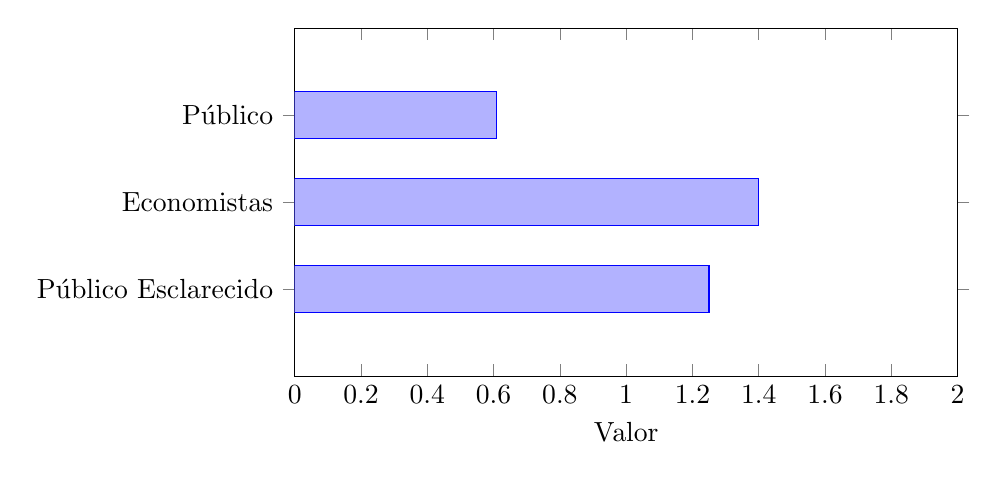
\begin{tikzpicture}
        \begin{axis}[
            xbar,
            symbolic y coords={Público, Economistas, Público Esclarecido},
            ytick=data,
            xmin=0, xmax=2,
            xlabel={Valor},
            bar width=0.6cm,
            width=10cm,
            height=6cm,
            enlarge y limits=0.5,
            y dir=reverse % Invert the y-axis to maintain the desired order
        ]
        \addplot coordinates {(0.61,Público) (1.4,Economistas) (1.25,Público Esclarecido)};
        \end{axis}
    \end{tikzpicture}
    \caption{Elaborado pelo autor com base em Caplan (\citeyear{The_Myth_of_the_Rational_Voter}) \newline
    Nota: As respostas são dadas em uma escala de 0 a 2, onde 0 = “ruim”, 1 = “indiferente” e 2 = “bom”.}
    \label{fig:pergunta_23}
\end{figure}

Economistas não apenas veem os perigos da redução de postos de trabalho como algo exagerado, ele veem isso como uma coisa boa. A redução de postos de trabalho é um sinal de que a economia está se ajustando, de que os recursos estão sendo realocados para onde são mais necessários. Já o publico em geral, vê a redução de postos de trabalho como algo ruim. É preciso lembra-los que a economia é um sistema dinâmico, e que a destruição criativa é um processo necessário para o progresso econômico \cite{schumpeter1976capitalism}, fazer mais com menos é a definição de progresso econômico \cite{The_Myth_of_the_Rational_Voter}.



\begin{figure}[H]
    \centering
    \caption*{Pergunta 24: “Algumas pessoas dizem que estes são tempos economicamente instáveis por causa das novas tecnologias, da concorrência de países estrangeiros e da redução de pessoal. Olhando para os próximos 20 anos, você acha que essas mudanças serão, eventualmente, boas ou ruins para o país, ou você acha que essas mudanças não farão muita diferença?”}
    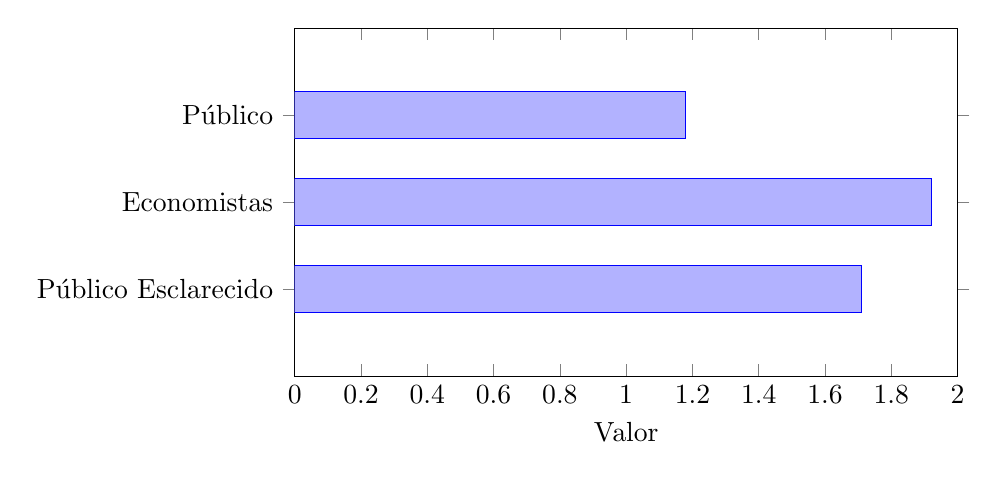
\begin{tikzpicture}
        \begin{axis}[
            xbar,
            symbolic y coords={Público, Economistas, Público Esclarecido},
            ytick=data,
            xmin=0, xmax=2,
            xlabel={Valor},
            bar width=0.6cm,
            width=10cm,
            height=6cm,
            enlarge y limits=0.5,
            y dir=reverse % Invert the y-axis to maintain the desired order
        ]
        \addplot coordinates {(1.18,Público) (1.92,Economistas) (1.71,Público Esclarecido)};
        \end{axis}
    \end{tikzpicture}
    \caption{Elaborado pelo autor com base em Caplan (\citeyear{The_Myth_of_the_Rational_Voter}) \newline
    Nota: As respostas são dadas em uma escala de 0 a 2, onde 0 = “ruim”, 1 = “indiferente” e 2 = “bom”.}
    \label{fig:pergunta_24}
\end{figure}

Para abordar a questão da discrepância entre especialistas e leigos na compreensão econômica, a explicação mais plausível pode ser atribuída às diferentes perspectivas temporais que cada grupo adota. Economistas tendem a focar no "longo prazo", enquanto a opinião pública se preocupa mais com as implicações imediatas. É possível que especialistas e o público compartilhem uma compreensão comum dos fatos, mas tenham diferentes níveis de paciência para os resultados.

Como Schumpeter observa: 

\begin{citacao}
    \textit{
        Reconhecer racionalmente o desempenho econômico do capitalismo e as esperanças que ele oferece para o futuro exigiria um feito moral quase impossível para os menos favorecidos. Esse desempenho se destaca apenas se adotarmos uma perspectiva de longo prazo; qualquer argumento a favor do capitalismo deve repousar sobre considerações de longo prazo. (...) Para as massas, o curto prazo é o que conta. Assim com Luís XV, elas podem dizer: “Depois de mim, o dilúvio”.  
    } \newline
    \cite{schumpeter1976capitalism}
\end{citacao}

Para testar a hipótese de Schumpeter, podemos analisar os efeitos esperados ao longo de 20 anos. Se as diferenças de paciência fossem a única explicação, leigos e especialistas teriam opiniões muito semelhantes. No entanto, a discrepância de crenças é notavelmente grande. Ambos os grupos têm uma visão menos negativa sobre o longo prazo, mas os economistas são mais positivos em relação ao presente e ao futuro. Enquanto os especialistas esperam que uma bênção mista se torne uma vantagem pura, o público tende a acreditar que um problema puro se dissipará com o tempo \cite{The_Myth_of_the_Rational_Voter}.


\begin{figure}[H]
    \centering
    \caption*{Pergunta 25: "Você acha que os acordos comerciais entre os Estados Unidos e outros países ajudaram a criar mais empregos nos EUA, ou eles custaram empregos aos EUA, ou eles não fizeram muita diferença?"}
    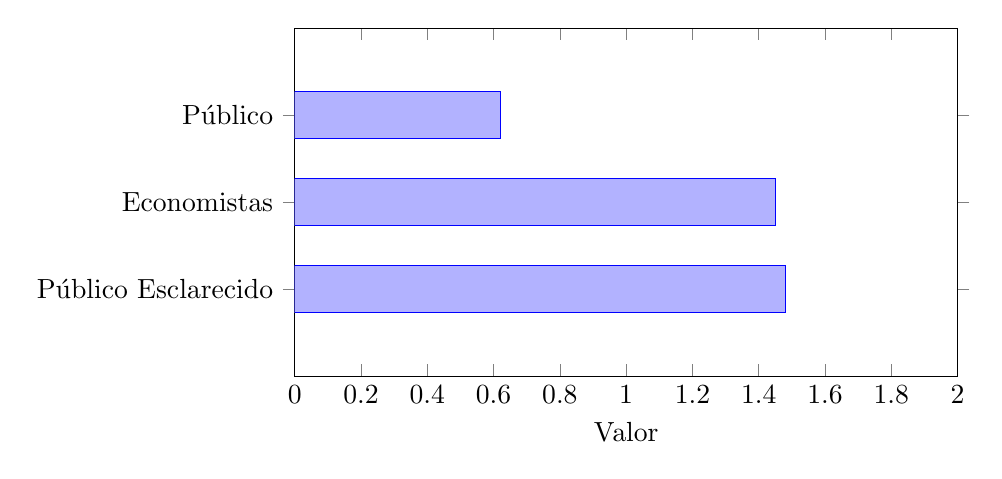
\begin{tikzpicture}
        \begin{axis}[
            xbar,
            symbolic y coords={Público, Economistas, Público Esclarecido},
            ytick=data,
            xmin=0, xmax=2,
            xlabel={Valor},
            bar width=0.6cm,
            width=10cm,
            height=6cm,
            enlarge y limits=0.5,
            y dir=reverse % Invert the y-axis to maintain the desired order
        ]
        \addplot coordinates {(0.62,Público) (1.45,Economistas) (1.48,Público Esclarecido)};
        \end{axis}
    \end{tikzpicture}
    \caption{Elaborado pelo autor com base em Caplan (\citeyear{The_Myth_of_the_Rational_Voter}) \newline
    Nota: As respostas são dadas em uma escala de 0 a 2, onde 0 = “custaram empregos”, 1 = “não fizeram diferença” e 2 = “ajudaram a criar empregos”.}
    \label{fig:pergunta_25}
\end{figure}

Quando a SAEE pergunta sobre o efeito dos acordos comerciais no emprego nos EUA, o viés antiestrangeiro e o viés antitrabalho se combinam, criando uma lacuna muito ampla entre economistas e o público. Independentemente da opinião geral dos não economistas sobre os acordos comerciais, eles estão convencidos de que o efeito sobre o emprego doméstico é negativo. Economistas e o público mais esclarecido negam essa visão, como era de se esperar.

Neste tipo de visão, economistas que preveem ganhos de empregos podem estar exagerando. A liberalização do comércio aumenta a demanda externa, mas reduz a demanda interna. Portanto, há poucas razões para esperar um benefício no emprego a curto prazo. Um efeito a longo prazo é ainda menos provável, uma vez que macroeconomistas duvidam que choques de demanda tenham efeitos duradouros no emprego \cite{blinder1987hard}. A resposta teoricamente fundamentada é focar nos padrões de vida, e não no emprego \cite{The_Myth_of_the_Rational_Voter}. 

\subsubsection{Diversas}

As questões restantes variam em forma e conteúdo, mas continuam a exibir grandes e robustas diferenças sistemáticas de crença.

\begin{figure}[H]
    \centering
    \caption*{Pergunta 26: “Quem você acha o maior responsável pelo aumento recente no preços dos combustíveis”}
    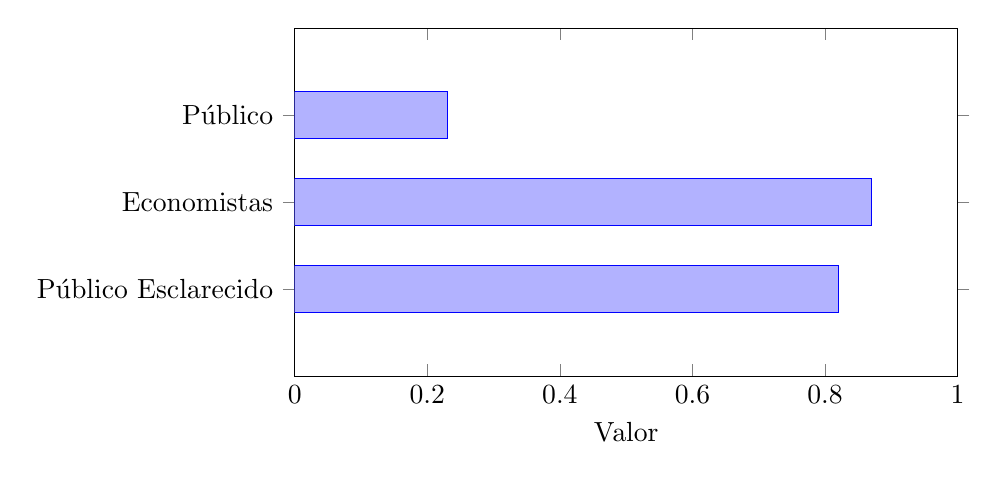
\begin{tikzpicture}
        \begin{axis}[
            xbar,
            symbolic y coords={Público, Economistas, Público Esclarecido},
            ytick=data,
            xmin=0, xmax=1,
            xlabel={Valor},
            bar width=0.6cm,
            width=10cm,
            height=6cm,
            enlarge y limits=0.5,
            y dir=reverse % Invert the y-axis to maintain the desired order
        ]
        \addplot coordinates {(0.23,Público) (0.87,Economistas) (0.82,Público Esclarecido)};
        \end{axis}
    \end{tikzpicture}
    \caption{Elaborado pelo autor com base em Caplan (\citeyear{The_Myth_of_the_Rational_Voter}) \newline
    Nota: As respostas são dadas em uma escala de 0 a 1, onde 0 = “Petrolíferas tentando aumentar lucros”, 1 = “Lei de oferta e demanda”.}
    \label{fig:pergunta_26}
\end{figure}

Uma forma chave de viés antimercado é negar ou minimizar o papel da competição. É revelador, portanto, que os economistas atribuam amplamente o aumento do preço da gasolina em 1996 às forças de oferta e demanda, enquanto apenas um quarto do público concorda com essa visão. Onde os economistas veem os preços determinados pelas forças de mercado, o público vê monopólio ou conluio. Os dados para o Público esclarecido confirmam que os economistas não discordam apenas porque são ricos demais para se preocupar com o custo de encher o tanque de gasolina.

O verdadeiro problema não é que os economistas estejam desconectados, mas que a narrativa do público não faz sentido. Se os preços da gasolina aumentam porque “as empresas de petróleo estão tentando aumentar seus lucros,” por que os preços da gasolina algum dia caem? As empresas de petróleo se tornam generosas e decidem reduzir seus lucros? A economia básica, em contraste, oferece uma explicação elegante: se o custo dos insumos diminui, o preço que maximiza o lucro também diminui. Se o custo dos insumos aumenta, o preço que maximiza o lucro também aumenta. A explicação do público é uma teoria da conspiração, não uma teoria econômica \cite{The_Myth_of_the_Rational_Voter}.

\begin{figure}[H]
    \centering
    \caption*{Pergunta 27: “Você acha que os preços dos combustíveis são altos demais, baixos demais ou no nível certo?”}
    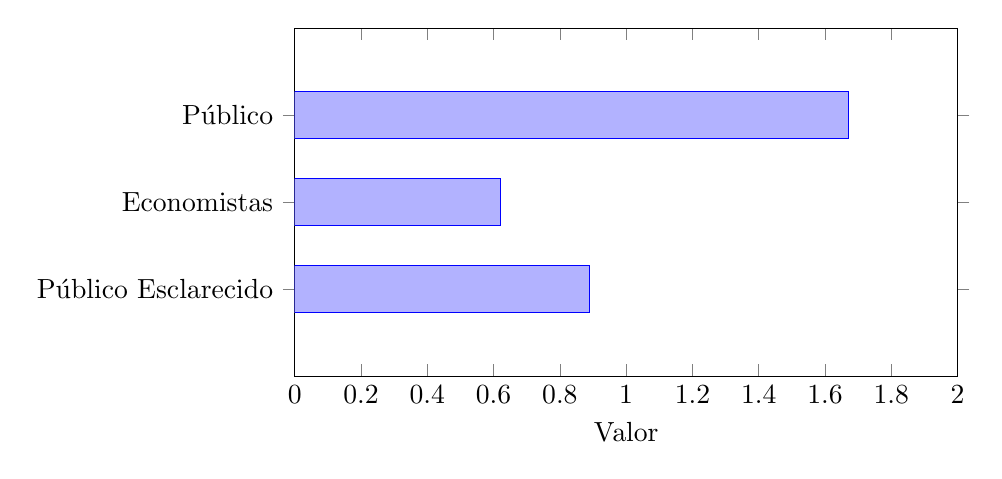
\begin{tikzpicture}
        \begin{axis}[
            xbar,
            symbolic y coords={Público, Economistas, Público Esclarecido},
            ytick=data,
            xmin=0, xmax=2,
            xlabel={Valor},
            bar width=0.6cm,
            width=10cm,
            height=6cm,
            enlarge y limits=0.5,
            y dir=reverse % Invert the y-axis to maintain the desired order
        ]
        \addplot coordinates {(1.67,Público) (0.62,Economistas) (0.89,Público Esclarecido)};
        \end{axis}
    \end{tikzpicture}
    \caption{Elaborado pelo autor com base em Caplan (\citeyear{The_Myth_of_the_Rational_Voter}) \newline
    Nota: As respostas são dadas em uma escala de 0 a 2, onde 0 = “baixos”, 1 = “nível certo” e 2 = “altos”.}
    \label{fig:pergunta_27}
\end{figure}

A formulação da questão 27 deixa a desejar; como consumidor, pode-se trivialmente considerar que qualquer preço é “muito alto.” No entanto, as respostas à questão anterior sugerem que poucos respondentes interpretam a pergunta de forma tão literal. Quando as pessoas respondem “muito alto,” provavelmente querem dizer que algum tipo de monopólio mantém os preços acima do nível competitivo. Por outro lado, “muito baixo” provavelmente significa que impostos mais elevados sobre combustíveis são necessários para corrigir a poluição, congestionamento e outras externalidades negativas do uso de automóveis.

A posição de “muito alto” é uma forma clássica de viés antimercado. No entanto, a oposição à tese de “muito baixo” pode, arguivelmente, ter a mesma raiz. Suponha que você queira reduzir a poluição e o congestionamento. Você poderia fazer isso por meio de um comando e controle: regulamentações de emissões, inspeções anuais, faixas para caronas. Mas os economistas reconhecem que o mecanismo de mercado é um método mais eficiente. Um imposto sobre a gasolina oferece às pessoas um incentivo para reduzir a poluição e o congestionamento sem ditar especificamente o comportamento de ninguém \cite{The_Myth_of_the_Rational_Voter,blinder1987hard}.


\begin{figure}[H]
    \centering
    \caption*{Pergunta 28: “Você acha que o presidente pode fazer muito, pouco ou que está além da capacidade de ele melhorar a economia”}
    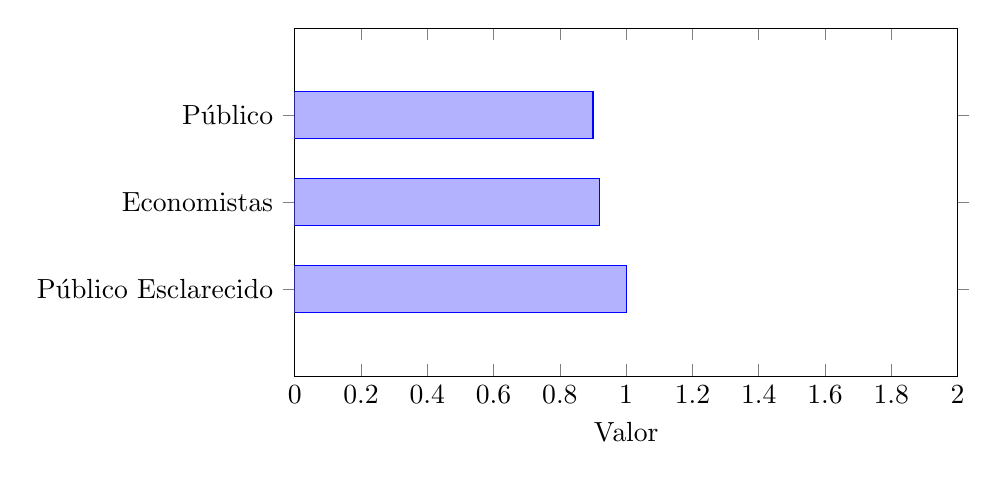
\begin{tikzpicture}
        \begin{axis}[
            xbar,
            symbolic y coords={Público, Economistas, Público Esclarecido},
            ytick=data,
            xmin=0, xmax=2,
            xlabel={Valor},
            bar width=0.6cm,
            width=10cm,
            height=6cm,
            enlarge y limits=0.5,
            y dir=reverse % Invert the y-axis to maintain the desired order
        ]
        \addplot coordinates {(0.90,Público) (0.92,Economistas) (1,Público Esclarecido)};
        \end{axis}
    \end{tikzpicture}
    \caption{Elaborado pelo autor com base em Caplan (\citeyear{The_Myth_of_the_Rational_Voter}) \newline
    Nota: As respostas são dadas em uma escala de 0 a 2, onde 0 = “além da capacidade”, 1 = “pode fazer pouco” e 2 = “pode fazer muito”.}
    \label{fig:pergunta_28}
\end{figure}

Uma questão rara em que economistas e o público concordam é sobre a capacidade do presidente de melhorar a economia. Isso é especialmente curioso porque os economistas criticam o público por associar mecanicamente as condições econômicas aos presidentes em exercício. E quanto ao Federal Reserve, ao Congresso, a outros governos, às tendências seculares e aos choques aleatórios? Quando os economistas criticam apenas erros em uma direção, geralmente há uma boa razão para isso: os erros nessa direção predominam. Este é o caso que confirma a regra. Talvez aqueles que minimizam a influência do presidente sejam menos expressivos, criando a ilusão de uma diferença sistemática.



\begin{figure}[H]
    \centering
    \caption*{Pergunta 29: “Você acha que os novos postos de trabalho do país pagam bem ou mal?”}
    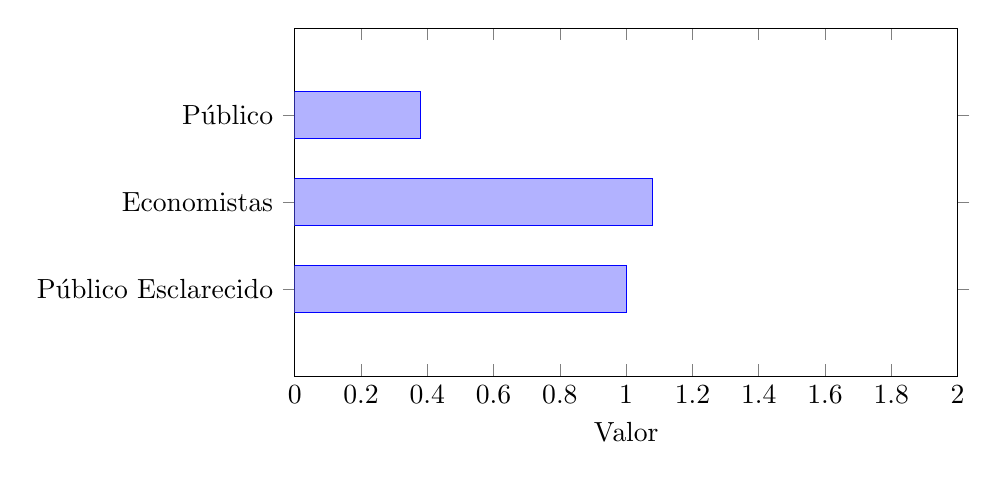
\begin{tikzpicture}
        \begin{axis}[
            xbar,
            symbolic y coords={Público, Economistas, Público Esclarecido},
            ytick=data,
            xmin=0, xmax=2,
            xlabel={Valor},
            bar width=0.6cm,
            width=10cm,
            height=6cm,
            enlarge y limits=0.5,
            y dir=reverse % Invert the y-axis to maintain the desired order
        ]
        \addplot coordinates {(0.38,Público) (1.08,Economistas) (1,Público Esclarecido)};
        \end{axis}
    \end{tikzpicture}
    \caption{Elaborado pelo autor com base em Caplan (\citeyear{The_Myth_of_the_Rational_Voter}) \newline
    Nota: As respostas são dadas em uma escala de 0 a 2, onde 0 = “pagam mal”, 1 = “nem uma coisa, nem outra” e 2 = “pagam bem”.}
    \label{fig:pergunta_29}
\end{figure}

A expectativa predominante do público tende a ser pessimista, refletindo a crença de que as condições econômicas estão inevitavelmente piorando. Desde a década de 1970, a percepção de estagnação e declínio tem dominado a narrativa econômica popular. Em contraste, os economistas frequentemente argumentam que os dados contrariam esse pessimismo extremo \cite{Myths-of-Rich-and-Poor}. No entanto, a disparidade de crenças vai além das estatísticas mais recentes. O progresso econômico dos últimos séculos sugere que é anômalo que novos empregos apresentem remunerações significativamente baixas. Embora um retrocesso temporário possa ocorrer, ele merece uma análise mais aprofundada para compreender sua natureza e implicações.



\begin{figure}[H]
    \centering
    \caption*{Pergunta 30: “Você acha que a desigualdade entre os ricos e os pobres é menor ou maior do que há vinte anos, ou é praticamente a mesma”}
    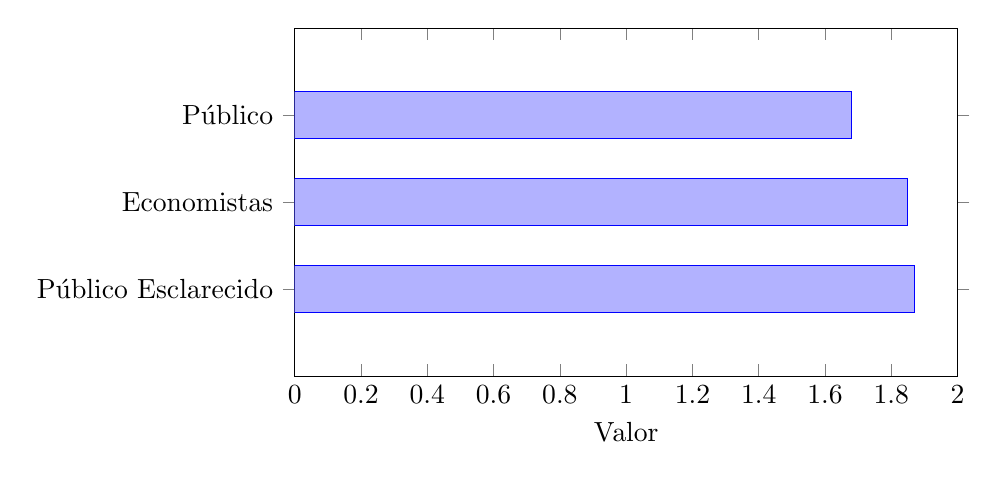
\begin{tikzpicture}
        \begin{axis}[
            xbar,
            symbolic y coords={Público, Economistas, Público Esclarecido},
            ytick=data,
            xmin=0, xmax=2,
            xlabel={Valor},
            bar width=0.6cm,
            width=10cm,
            height=6cm,
            enlarge y limits=0.5,
            y dir=reverse % Invert the y-axis to maintain the desired order
        ]
        \addplot coordinates {(1.68,Público) (1.85,Economistas) (1.87,Público Esclarecido)};
        \end{axis}
    \end{tikzpicture}
    \caption{Elaborado pelo autor com base em Caplan (\citeyear{The_Myth_of_the_Rational_Voter}) \newline
    Nota: As respostas são dadas em uma escala de 0 a 2, onde 0 = “menor”, 1 = “praticamente a mesma” e 2 = “maior”.}
    \label{fig:pergunta_30}
\end{figure}

O público percebe duas décadas de aumento da desigualdade. Dada sua tendência antimercado e pessimista, como poderia ser diferente? No entanto, contra a expectativa, os economistas estão mais convencidos do que o público. Os dados sobre desigualdade são suficientemente sólidos, e os economistas não possuem presunções fortes sobre a desigualdade \cite{Gottschalk-Peter}. Eles reconhecem que os padrões de vida aumentam ao longo do tempo, mas têm poucas razões para esperar uma tendência na distribuição de renda e riqueza \cite{The_Myth_of_the_Rational_Voter}.


\begin{figure}[H]
    \centering
    \caption*{Pergunta 31: “Nos últimos 20 anos, você acha que, em geral, as rendas familiares dos americanos médios têm aumentado mais rapidamente do que o custo de vida, têm se mantido aproximadamente no mesmo nível do custo de vida, ou têm ficado atrás do custo de vida?”}
    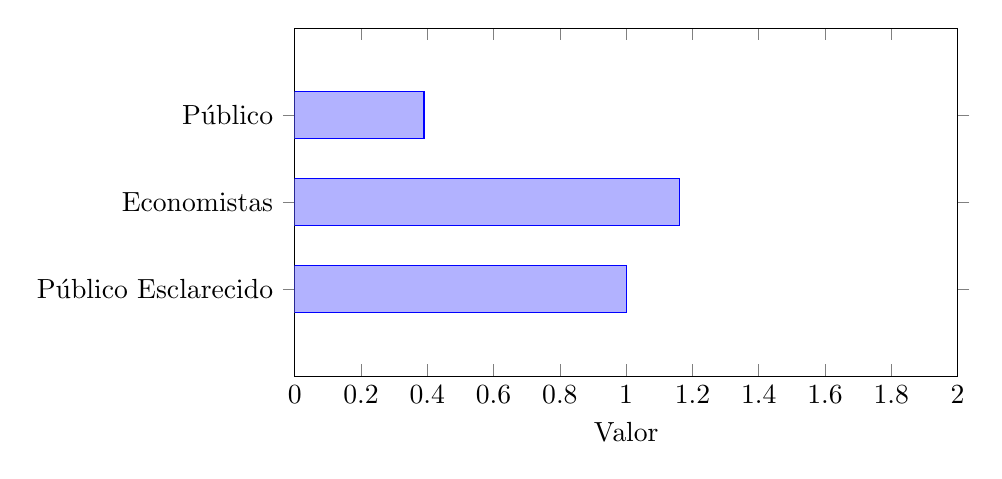
\begin{tikzpicture}
        \begin{axis}[
            xbar,
            symbolic y coords={Público, Economistas, Público Esclarecido},
            ytick=data,
            xmin=0, xmax=2,
            xlabel={Valor},
            bar width=0.6cm,
            width=10cm,
            height=6cm,
            enlarge y limits=0.5,
            y dir=reverse % Invert the y-axis to maintain the desired order
        ]
        \addplot coordinates {(0.39,Público) (1.16,Economistas) (1,Público Esclarecido)};
        \end{axis}
    \end{tikzpicture}
    \caption{Elaborado pelo autor com base em Caplan (\citeyear{The_Myth_of_the_Rational_Voter}) \newline
    Nota: As respostas são dadas em uma escala de 0 a 2, onde 0 = “ficou para trás”, 1 = “mesmo nível” e 2 = “cresceu mais rápido”.}
    \label{fig:pergunta_31}
\end{figure}

A interpretação do "viés pessimista" como uma questão meramente semântica é tentadora. Pode-se argumentar que o público observa que "a economia está indo mal em relação às suas expectativas pessoais," enquanto os economistas respondem que "a economia está indo bem, considerando suas limitações estruturais." No entanto, se o descompasso fosse apenas uma questão de terminologia, o pessimismo aparente se reduziria em temas menos ambíguos. Esse não é o caso. A questão relativa à renda familiar na SAEE, por ser uma das menos ambíguas, expõe uma das mais significativas lacunas de crença entre leigos e especialistas.

A lacuna de crença não deveria ser ainda mais acentuada? A média das respostas dos economistas é ligeiramente superior a 1; isso sugere que uma minoria substancial da profissão nega o aumento da renda média? Não é o caso. O fator complicador aqui é o aumento da desigualdade. A questão se refere à renda mediana (“renda familiar para os americanos típicos”), e não à renda média (“renda média das famílias americanas”). Em um contexto de crescente desigualdade, a renda mediana pode diminuir enquanto a renda média aumenta. Embora quase todos os economistas reconheçam a distinção entre renda média e mediana, é duvidoso que muitos não economistas compartilhem dessa compreensão. Os membros do público que afirmaram "estar ficando para trás" provavelmente acreditam que a renda média caiu entre 1976 e 1996. Contudo, mesmo os economistas que relataram "estar ficando para trás" são conscientes de que a renda média aumentou. Assim, a ambiguidade residual nesta questão obscurece a verdadeira magnitude da lacuna entre leigos e especialistas, subestimando a profundidade da discordância entre esses grupos \cite{The_Myth_of_the_Rational_Voter}.


\begin{figure}[H]
    \centering
    \caption*{Pergunta 32: “Pensando apenas nos salários do trabalhador americano médio, você acha que, nos últimos 20 anos, eles têm aumentado mais rapidamente do que o custo de vida, têm se mantido aproximadamente no mesmo nível do custo de vida, ou têm ficado atrás do custo de vida?”}
    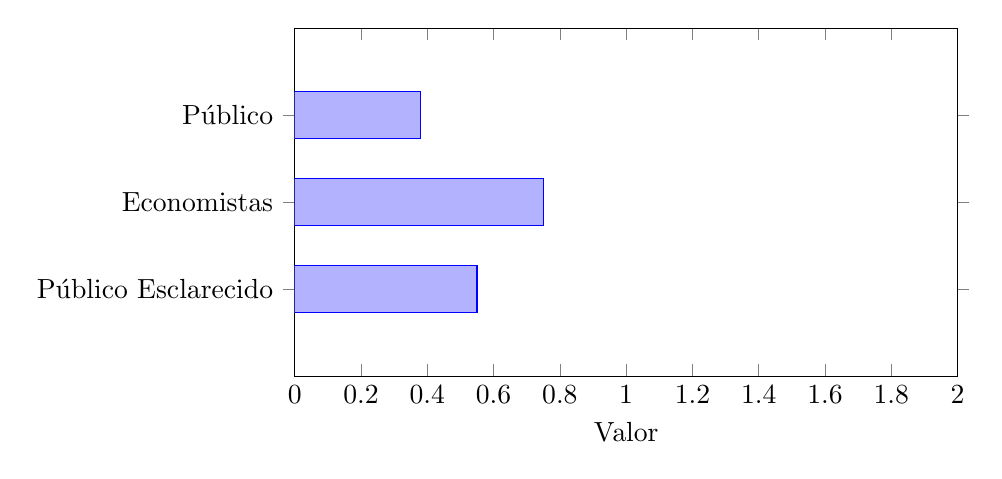
\begin{tikzpicture}
        \begin{axis}[
            xbar,
            symbolic y coords={Público, Economistas, Público Esclarecido},
            ytick=data,
            xmin=0, xmax=2,
            xlabel={Valor},
            bar width=0.6cm,
            width=10cm,
            height=6cm,
            enlarge y limits=0.5,
            y dir=reverse % Invert the y-axis to maintain the desired order
        ]
        \addplot coordinates {(0.38,Público) (0.75,Economistas) (0.55,Público Esclarecido)};
        \end{axis}
    \end{tikzpicture}
    \caption{Elaborado pelo autor com base em Caplan (\citeyear{The_Myth_of_the_Rational_Voter}) \newline
    Nota: As respostas são dadas em uma escala de 0 a 2, onde 0 = “ficou para trás”, 1 = “mesmo nível” e 2 = “cresceu mais rápido”.}
    \label{fig:pergunta_32}
\end{figure}

A lacuna de crença em relação aos salários reais é significativamente mais estreita do que a observada para a renda real, com essa mudança sendo quase inteiramente atribuível aos economistas. O público tende a oferecer respostas semelhantes em ambas as questões, possivelmente porque confunde renda e salários. Os economistas, por sua vez, compreendem que são conceitos distintos e reconhecem que alguns dados sobre os salários reais médios contradizem a presunção de progresso contínuo. Se os salários reais médios permanecem estagnados enquanto a desigualdade aumenta, é razoável inferir que os salários do trabalhador médio estão diminuindo. No entanto, uma minoria substancial de economistas ainda sustenta a presunção de progresso salarial, apontando para sérias falhas que tendem a reduzir as estimativas oficiais \cite{Myths-of-Rich-and-Poor}.

\begin{figure}[H]
    \centering
    \caption*{Pergunta 33: “Algumas pessoas dizem que, para ter uma vida confortável, a família média deve ter dois assalariados em tempo integral. Você concorda com isso, ou acha que a família média pode viver confortavelmente com apenas um assalariado em tempo integral?”}
    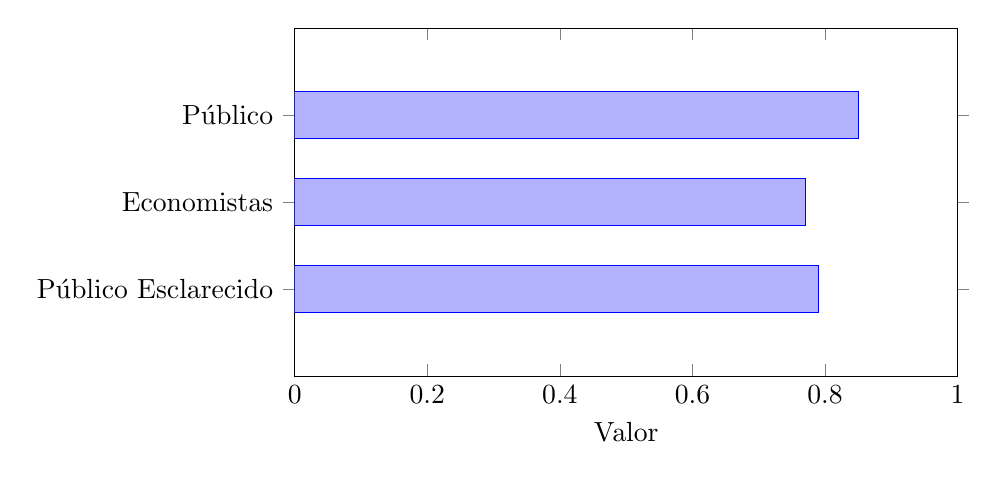
\begin{tikzpicture}
        \begin{axis}[
            xbar,
            symbolic y coords={Público, Economistas, Público Esclarecido},
            ytick=data,
            xmin=0, xmax=1,
            xlabel={Valor},
            bar width=0.6cm,
            width=10cm,
            height=6cm,
            enlarge y limits=0.5,
            y dir=reverse % Invert the y-axis to maintain the desired order
        ]
        \addplot coordinates {(0.85,Público) (0.77,Economistas) (0.79,Público Esclarecido)};
        \end{axis}
    \end{tikzpicture}
    \caption{Elaborado pelo autor com base em Caplan (\citeyear{The_Myth_of_the_Rational_Voter}) \newline
    Nota: As respostas são dadas em uma escala de 0 a 2, onde 0 = "pode viver com um assalariado" e 1 = "precisa de dois assalariados".}
    \label{fig:pergunta_33}
\end{figure}

Grandes maiorias tanto de economistas quanto do público concordam que a família americana média necessita de duas rendas para viver confortavelmente, embora os economistas sejam menos categóricos. Essa diferença não reflete a renda acima da média dos economistas, pois o Público Esclarecido também compartilha dessa opinião. A provável razão para o menor pessimismo dos economistas é a prática do pensamento marginal. Ser uma mãe que fica em casa ou ter um emprego em tempo integral não são as únicas opções. Uma renda menor implica alguns sacrifícios, mas uma família com um provedor em tempo integral e outro em meio período pode se ajustar "confortavelmente" de várias maneiras: comprar uma casa moderadamente mais barata ou adiar a compra de um carro novo por um ou dois anos \cite{The_Myth_of_the_Rational_Voter}.


\begin{figure}[H]
    \centering
    \caption*{Pergunta 34: “Nos próximos cinco anos, você acha que o padrão de vida do americano médio vai subir, cair ou se manter aproximadamente o mesmo?”}
    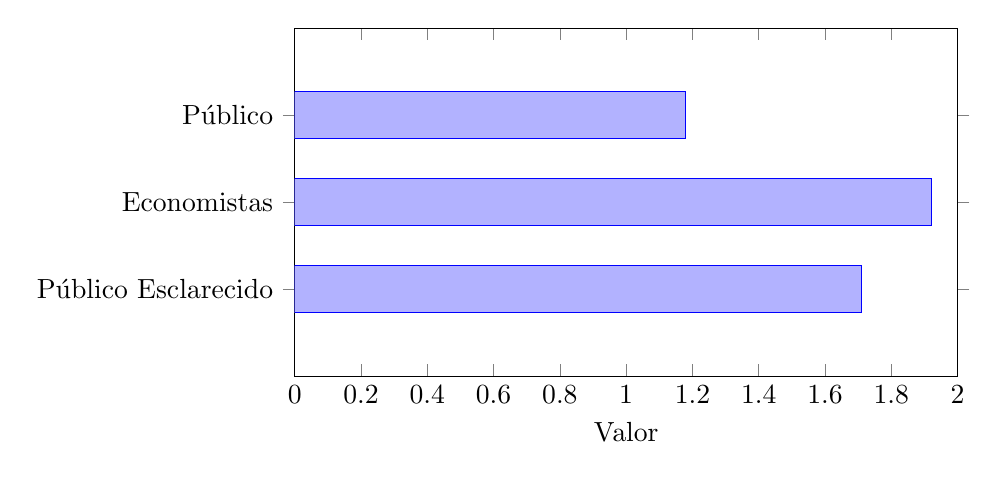
\begin{tikzpicture}
        \begin{axis}[
            xbar,
            symbolic y coords={Público, Economistas, Público Esclarecido},
            ytick=data,
            xmin=0, xmax=2,
            xlabel={Valor},
            bar width=0.6cm,
            width=10cm,
            height=6cm,
            enlarge y limits=0.5,
            y dir=reverse % Invert the y-axis to maintain the desired order
        ]
        \addplot coordinates {(1.18,Público) (1.92,Economistas) (1.71,Público Esclarecido)};
        \end{axis}
    \end{tikzpicture}
    \caption{Elaborado pelo autor com base em Caplan (\citeyear{The_Myth_of_the_Rational_Voter}) \newline
    Nota: As respostas são dadas em uma escala de 0 a 2, onde 0 = "cair", 1 = "se manter aproximadamente o mesmo" e 2 = "subir".}
    \label{fig:pergunta_34}
\end{figure}

Com dados suficientes, é possível convencer um economista de que melhorias nos padrões de vida não se materializaram em algum momento do passado ou que uma recessão iminente irá reduzi-los. No entanto, é difícil fazer um economista deixar de esperar por padrões de vida em ascensão no médio ou longo prazo. Críticos veem isso como prova de seu dogmatismo. Contudo, a presunção de progresso não surge do nada. Dois séculos de impressionante crescimento econômico a sustentam \cite{catching-up,making-a-miracle,Pursuing-Happiness}. Não é mais dogmático que os não economistas permaneçam pessimistas apesar desse histórico? 


\begin{figure}[H]
    \centering
    \caption*{Pergunta 35: “Você espera que a geração de seus filhos desfrute de um padrão de vida mais alto ou mais baixo do que a sua geração, ou acha que será aproximadamente o mesmo?”}
    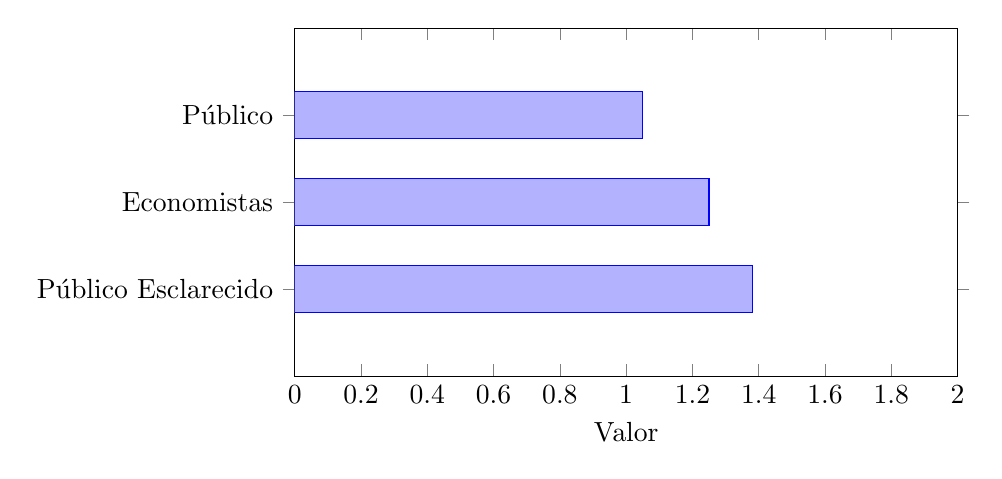
\begin{tikzpicture}
        \begin{axis}[
            xbar,
            symbolic y coords={Público, Economistas, Público Esclarecido},
            ytick=data,
            xmin=0, xmax=2,
            xlabel={Valor},
            bar width=0.6cm,
            width=10cm,
            height=6cm,
            enlarge y limits=0.5,
            y dir=reverse % Invert the y-axis to maintain the desired order
        ]
        \addplot coordinates {(1.05,Público) (1.25,Economistas) (1.38,Público Esclarecido)};
        \end{axis}
    \end{tikzpicture}
    \caption{Elaborado pelo autor com base em Caplan (\citeyear{The_Myth_of_the_Rational_Voter}) \newline
    Nota: As respostas são dadas em uma escala de 0 a 2, onde 0 = "mais baixo", 1 = "aproximadamente o mesmo" e 2 = "mais alto".}
    \label{fig:pergunta_35}
\end{figure}

Aqui está um exemplo ideal de pergunta para sondar as crenças dos respondentes sobre o crescimento de longo prazo. As crenças dos economistas sobre o futuro econômico são naturalmente mais otimistas do que as dos não economistas, embora a diferença seja menor do que se poderia esperar. Surpreendentemente, o Público Esclarecido é mais otimista do que ambos. A razão é que homens de alta renda são atipicamente pessimistas sobre esse tópico. Como os economistas tendem a ser homens de alta renda, suas características demográficas atenuam seu otimismo \cite{The_Myth_of_the_Rational_Voter}.


\begin{figure}[H]
    \centering
    \caption*{Pergunta 36: [Se você tem filhos com menos de 30 anos] "Quando eles atingirem a sua idade, você espera que eles desfrutem de um padrão de vida mais alto ou mais baixo do que o seu agora, ou espera que seja aproximadamente o mesmo?”}
    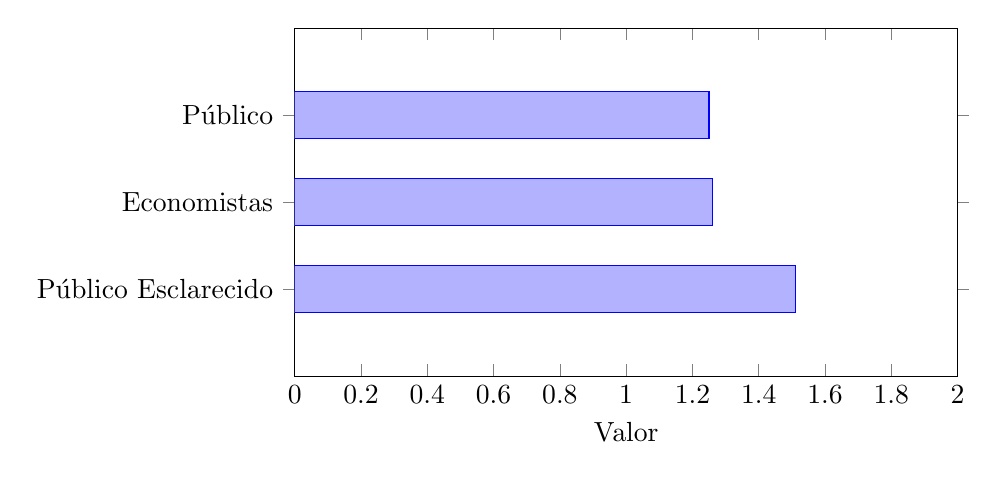
\begin{tikzpicture}
        \begin{axis}[
            xbar,
            symbolic y coords={Público, Economistas, Público Esclarecido},
            ytick=data,
            xmin=0, xmax=2,
            xlabel={Valor},
            bar width=0.6cm,
            width=10cm,
            height=6cm,
            enlarge y limits=0.5,
            y dir=reverse % Invert the y-axis to maintain the desired order
        ]
        \addplot coordinates {(1.25,Público) (1.26,Economistas) (1.51,Público Esclarecido)};
        \end{axis}
    \end{tikzpicture}
    \caption{Elaborado pelo autor com base em Caplan (\citeyear{The_Myth_of_the_Rational_Voter}) \newline
    Nota: As respostas são dadas em uma escala de 0 a 2, onde  0 = "mais baixo", 1 = "aproximadamente o mesmo" e 2 = "mais alto".}
    \label{fig:pergunta_36}
\end{figure}

Parece especialmente estranho que economistas e o público concordem sobre o futuro econômico de seus próprios filhos. Se os economistas são mais otimistas do que o público em relação às perspectivas da próxima geração, por que os dois grupos são igualmente otimistas em relação aos seus próprios filhos? Uma análise mais detalhada revela que os economistas são, de fato, mais otimistas, especialmente quando se controla pela renda \cite{The_Myth_of_the_Rational_Voter}. Se uma pessoa de meios modestos tivesse a educação de um economista, ela veria um futuro mais brilhante para seus filhos. Há uma explicação lógica para esse padrão. A questão pede que os respondentes comparem sua situação atual com a de seus filhos. Quanto melhor a sua situação, mais bem-sucedidos seus filhos precisam ser para igualá-lo. Muitos respondentes do SAEE parecem compreender esse ponto sutil: à medida que a renda aumenta, o otimismo diminui acentuadamente. O resultado é que a renda dos economistas camufla seu otimismo.



\begin{figure}[H]
    \centering
    \caption*{Pergunta 37: “Quando você pensa na economia dos Estados Unidos hoje, você acha que ela está...”}
    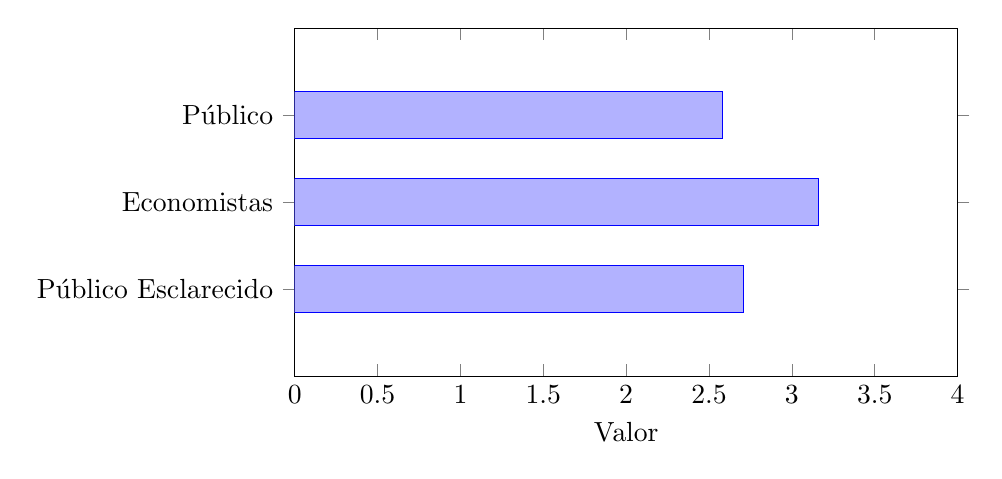
\begin{tikzpicture}
        \begin{axis}[
            xbar,
            symbolic y coords={Público, Economistas, Público Esclarecido},
            ytick=data,
            xmin=0, xmax=4,
            xlabel={Valor},
            bar width=0.6cm,
            width=10cm,
            height=6cm,
            enlarge y limits=0.5,
            y dir=reverse % Invert the y-axis to maintain the desired order
        ]
        \addplot coordinates {(2.58,Público) (3.16,Economistas) (2.71,Público Esclarecido)};
        \end{axis}
    \end{tikzpicture}
    \caption{Elaborado pelo autor com base em Caplan (\citeyear{The_Myth_of_the_Rational_Voter}) \newline
    Nota: As respostas são dadas em uma escala de 0 a 2, onde 0 = "em depressão", 1 = "em recessão", 2 = "estagnando", 3 = "crescendo lentamente" e 4 = "crescendo rapidamente".}
    \label{fig:pergunta_37}
\end{figure}

Quando perguntados sobre o estado atual da economia, os economistas dão respostas mais otimistas do que o restante do público. A raiz da discordância não é, contudo, o treinamento econômico. Os economistas têm a mesma opinião que os não economistas que possuem alta segurança no emprego e rendas crescentes. Após controlar essas características, a lacuna de crença deixa de ser estatisticamente significativa \cite{The_Myth_of_the_Rational_Voter}.


\subsubsection{A dúvida sobre a eficácia da SAEE}

As descobertas feitas a partir da SAEE por autores como Caplan, Miller e outros, embora não sejam infalíveis, são muito bem fundamentadas e amplamente aceitas na comunidade acadêmica. Uma das principais críticas que podem surgir em relação à ideia de que "os especialistas estão certos e os leigos, errados" é a imprecisão das perguntas formuladas. Termos como "muito" e "pouco", quando utilizados para definir as razões do baixo desempenho econômico, são vagos e podem resultar em respostas ambíguas, levando a conclusões potencialmente imprecisas.

Além disso, deve-se considerar a possível falta de sinceridade dos respondentes. A SAEE mede o que as pessoas dizem acreditar, não necessariamente o que realmente acreditam. É plausível que, ao responder à pesquisa, os indivíduos estejam mais preocupados em parecer inteligentes ou politicamente corretos do que em expressar suas verdadeiras convicções, resultando em respostas desonestas. Como explica Gordon Tullock:

\begin{quote}
    \textit{
        "Um homem pode informar um cientista social que está tentando alcançar algum objetivo por um determinado curso de ação, embora o curso de ação não pareça bem escolhido à vista do objetivo declarado. Um cientista social incauto pode então concluir que o homem é irracional. A verdadeira explicação pode simplesmente ser que os objetivos almejados são diferentes dos objetivos declarados."
    }
    \cite{tullock1987politics}
\end{quote}

Como resumo geral, pode-se afirmar que "os economistas estão certos e os leigos, errados" é uma afirmação que, embora geralmente verdadeira, não é absoluta. Supomos que, quando um especialista e um leigo discordam, o especialista está mais próximo da verdade. No entanto, é importante reconhecer que especialistas também cometem erros. Portanto, é necessário ter sorte ao escolher criticar o especialista em vez do leigo, superando a suposição geral.

A citação de Gustavo Franco ilustra bem essa questão: "Ir contra o senso comum é um esporte radical: há muito risco e, se você errar, vai acabar no hospital." Essa observação sublinha os riscos inerentes a desafiar o consenso estabelecido.

Apesar disso, é comum criticar economistas utilizando variações do viés autoindulgente e do viés ideológico. No entanto, essas críticas frequentemente carecem de fundamentação robusta. A SAEE revela que essas duas críticas são, em grande parte, infundadas, pois os especialistas tendem a estar mais alinhados com a realidade dos fatos do que os leigos.






\newpage

\subsection{Brasil}

A análise dos vieses e preferências por crenças no Brasil também é rica e diversificada. Embora não tão extensa quanto nos Estados Unidos, os autores Claudio Djissey Shikida, Ari Francisco Araujo Jr e Andressa Mielke Vasconcelos, realizaram uma pesquisa semelhante à SAEE, na tentativa de compreender as diferenças nas crenças sobre a economia entre o público em geral e os economistas brasileiros.

A estrutura da pesquisa no Brasil inclui um conjunto de dados com n = 373, adotando como estratégia alternativa a utilização do sistema Google Formulários para que fosse replicado com algumas adaptações para o contexto brasileiro atual. Os entrevistados incluem uma amostra representativa da população brasileira e um grupo de economistas selecionados com base em sua especialização em política econômica.



\section{Interpretação dos Resultados e Implicações}

\section{Conclusão}

